\documentclass[12 pt, a4paper]{article}
\usepackage[english]{babel}  								% For norsk oppsett
\usepackage[utf8]{inputenc}
\usepackage{amsmath}
\usepackage{amssymb}
\usepackage{graphicx}
\usepackage{tabularx}
\usepackage{subcaption}
\usepackage{hyperref}
\usepackage{fancyhdr}
\usepackage{enumerate}
\usepackage{float}
\usepackage{tikz}
\usepackage{fancyhdr}
\usepackage{lastpage}
\usepackage{circuitikz}
\usepackage{physics}
\usepackage[includeheadfoot, margin =0.5 in]{geometry}
\usepackage[FYS, OnlyFrontpage]{mnfrontpage} 			%SKIFT HER!!!
\usepackage[version=3]{mhchem}
\usepackage{biblatex}%,style=numeric-comp
%\usepackage{cite}
\usepackage{siunitx}
\usepackage{todonotes}
\usepackage{xcolor}
\usepackage{listings}
%%%%
\usepackage[bottom]{footmisc}
\renewcommand\footnoterule{\rule{\linewidth}{0.5pt}}
%\renewcommand[\footnoterule]{%
%	\kern -3pt
%	\hrule width \textwidth height 1pt 
%	\kern 2pt
%}
%%%%
\lstset{basicstyle=\ttfamily,
  showstringspaces=false,
  commentstyle=\color{red},
  keywordstyle=\color{blue}
}
%\usepackage{showframe}  %Dette viser hvordan strukturen på sidene er

\setlength{\parindent}{0cm}

\author{
\href{https://scontent.fosl1-1.fna.fbcdn.net/v/t31.0-8/12671762_10153383742266712_8474119290530634136_o.jpg?oh=22ee31dac1e3bff8a581f96848315dbc&oe=5A7942F3}{Erik Skaar}
}



\bibliography{kilder.bib}






\font\myfont=cmr12 at 35pt
\title{\textbf{{\myfont Monte Carlo Modeling of Transactions}}}
\begin{document}
\mnfrontpage


\pagestyle{fancy}
\fancyhf{}
\rhead{FYS3150/FYS4150}
\lhead{\href{https://github.com/erikfsk/Project-5}{Erik Skaar,Thomas Storaas \& Mikael Kiste}}
\fancyfoot[CE,LO]{\leftmark}
\fancyfoot[LE,RO]{Page \number\value{page} of \pageref{LastPage}}

\renewcommand{\headrulewidth}{2pt}
\renewcommand{\footrulewidth}{1pt}

\tableofcontents


\pagebreak
\section*{Abstract}%1

\abstract{I this project a model of a financial marked is build up from the basics, and follows two papers written on financial models. Three additional different levels of complexity is added to the system to expand the model. First the system only consists of agents that has to trade with each other. The resulting plots from this model is then compared to Pareto's law to verify the models basics. Then a savings term is introduced and several different savings factors are compared to make a comment on how saving influences the money distribution. Then a probability is added to the transaction stage. Here people with a similar amount of money are more willing to do a transaction. A scaling power factor is introduced and varied to influence to what extend the similarity in wealth influences the probability to trade. Here the results are commented and compared to Pareto's law. Finally a trust term is included in the probability term. This term increases the probability of making a transaction if the agents has previously done transactions. This term also has a scaling power factor which is varied to compare the influence of this term on the final wealth distribution. Lastly a modification is done to one of the scaling factors compared to the one in the papers followed in this project.}




\section{Introduction}

Predictions of how the financial marked works has, in the modern age, become a large field of study\cite{publisher}. With the knowledge of how stock exchanges work can a mathematical model be build up to simulate these exchanges in the hope that one can predict prices and trends in the future. These predictions are in turn used as a basis for investments and such. The accuracy and speed of these models are therefore of the utmost importance. When these models predicts the wrong outcome things can go very wrong as it did in 2009\cite{marketcrash}.\\

In this project a simulation is done on a simple closed economy model. The economy model consists of a group of financial agents with the ability to transfer money between themselves, using the Monte Carlo method. The simulation will be compared to the well established Pareto's law \cite{paretoslaw}, and the analysis follows two papers. Patriarca with collaborates made one of the articles.\cite{patriarca} The second one was written by Goswami and Sen. \cite{goswami}

In the first simulation all financial agents are made equal and there is a $100\%$ probability of a transaction taking place when a trade is suggested. This it the simplest case and the model is then compared with a logarithmic plot to verify the trend. Then complexity is added by introducing saving. The model is further refined by adding a willingness to trade with agents with a comparative wealth to themselves. Lastly a favorable bias towards agents in which a trade has happened before is added. The whole job will be parallelized to speed up the simulations.\\


\todo[inline]{legg til noe mer for å dekke en side?}



















































\pagebreak
\section{Physical theory}\label{sec:phys-theory}
\subsection{Basics}\label{sec:basics}

 From empirical studies Pareto has been shown that the higher end of a distribution of money follows the distribution trend\cite{paretoslaw}:
 \begin{align}
 	\omega_m\propto m{-1-\alpha}\label{eq:pareto}
 \end{align} 
Here $\alpha\in[1,2]$. This trend will be analytically studied with a system of micro dynamical relations between a group of financial agents, and the resulting money distribution between them. \\


The system consists of $N$ financial agents. They transfer money between them in pairs of $(i,j)$ and they all start with a fixed amount of money $m_0$. The amount of money is arbitrary. So in this project the amount of money is given in amount of "wealth". Here one wealth is $m_0$ and the symbol used is $\$$. A result from this is that $\langle m\rangle=1\$ $\\

At a time step a pair of agents, $(i,j)$, are chosen at random and let them transact money from $j$ to $i$. The pair is chosen at random so for a specific pair $m_i,m_j$ both $(m_i,m_j)$ and $(m_j,m_i)$ are possible. Money is conserved during the transaction which means that the money $\Delta m$ transfered from $j$ to $i$ has to be equal. This means that the total expression for the transaction can be writen as

\begin{align}
	m_i+m_j=m_i'+m_j'\label{eq:pengerbevart}
\end{align}

This transfer is done by a Randomized Number Generator and in this model none of the agents are left with a debt. To remove the debt from the picture, only a percentage of the money is transfered in stead of a fixed amount.

\begin{align}
	m_j'=\epsilon(m_i+m_j)&&\epsilon\in[0,1]\label{epsiloncrit}
\end{align}

And similar for $m_i'$.
\begin{align*}
	m_j'=(1-\epsilon)(m_i+m_j)&&\epsilon\in[0,1]
\end{align*}

Due to the limitations of $\epsilon$ no agent gets debt, but it is likley that one agent is left with zero $m\geq0$. This system now consists of a conserved amount of money with a transfer criteria. It can be shown that this system, given enough time, will relax towards a Gibbs distribution.\cite{proofgibbsdist}

\begin{align}
	\omega_m=\beta e^{-\beta m}
\end{align}

With

\begin{align}
	\beta=\frac{1}{\langle m\rangle}=\qty[\sum_i\frac{m_i}{N}]^{-1}\label{eq:beta}
\end{align}

This model uses $N=500$. The $500$ agents has to do enough transaction to achieve the above outlined distribution. The article suggests that $10^7$ transactions is enough. \cite{patriarca} To find the final equilibrium distribution $\omega_m$ $10^4$ runs were done and $\omega_m$ was taken as the average of all the recorded $\omega_m$. The distribution of agents is exponential, so plotting the logarithm of the trend should yield a straight line.
\begin{align*}
	\ln(\omega_m)=\ln(\beta e^{-\beta m})\\
	\ln(\omega_m)=\ln(\beta)-\beta m %\label{logarithmicline}
\end{align*}


\subsection{Savings}
\label{sec:savings}

To make the model more realistic complexity is added though a savings term. Now every agent will save a fraction of their wealth $\delta$ before the transaction takes place. The addition of this term will change the distribution of agents so it no longer makes a gibbs distribution.

\begin{align}
	m_i'=\lambda m_i+\epsilon(1-\lambda)(m_i+m_j)\label{savingsterm1}
\end{align}

and similar for $m_j'$.
 
 \begin{align}
	 m_j'=\lambda m_j+(1-\epsilon)(1-\lambda)(m_i+m_j) \label{savingsterm2}
 \end{align}
 
 The two terms in the expressions can be simplified by gathering both the savings term and the trading term in a variable $\delta m=(1-\lambda)(\epsilon m_j-(1-\epsilon)m_i)$
 
 \begin{align*}
	 m_i'=\lambda m_i+\delta m
 \end{align*}
 \begin{align*}
	 m_j'=\lambda m_j+\delta m
 \end{align*}

\subsection{Willingness to trade}

The model has up until now only varied how much is saved and not touched on if they want to trade. From observations it is know that the willingness to trade impacts if a trade takes place or not. Further refinement of the model includes two terms to include in the probability of trading. For this the model follows the work of.\cite{goswami} The model now takes into account that there is a probability

\begin{align}
	p_{ij}\propto \abs{m_i-m_j}^{-\alpha}\label{eq:willingness}
\end{align}

for an interaction to take place between two agents with respectively $m_i$ and $m_j$ wealth. The variable $\alpha$ is larger than zero. If $\alpha$ is zero one get the same model as in section \ref{sec:savings}. Several runs will be done with varying $\alpha$ to analyze the effect of the probability term on the expression.

\subsubsection{Normalization}
\label{sec:normalization1}
The equation \ref{eq:willingness} is not normalized. If one chooses a value less than one the expression will blow up and the probability becomes larger than one.\\

\begin{figure}[H]
\centering
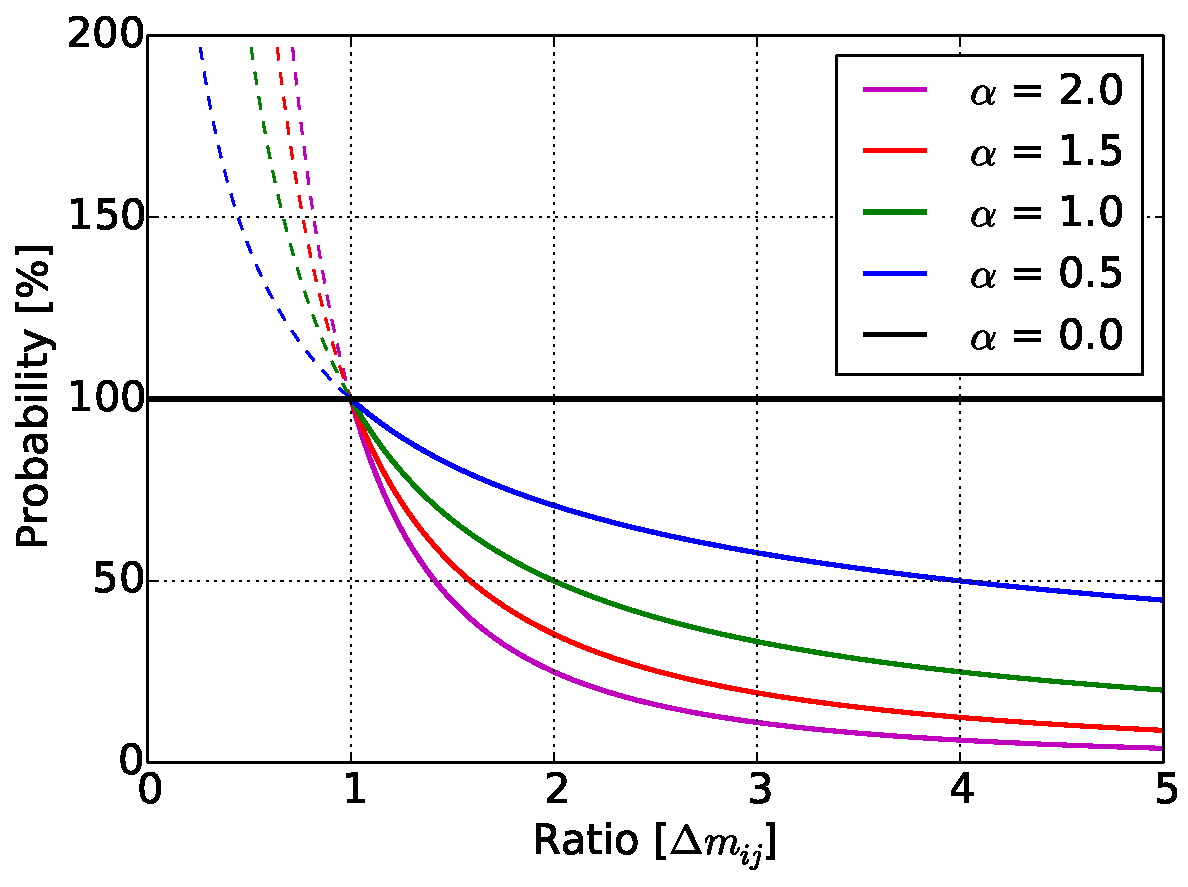
\includegraphics[width=0.7\linewidth]{theory/bilder/difference}
\caption{Figure shows the probability as a function of the difference in wealth between the two agents. The continuous line is the probability chosen in this project while the dashed line shows the trends without the criteria below one.}
\label{fig:difference}
\end{figure}


To prevent unrealistic probabilities above one a normalization criteria is introduced. The suggested normalization criteria on piazza is to normalize it with the expectation value of the agents $\langle m\rangle$.\footnote{\href{https://piazza.com/class/j6owewp05ym46p?cid=126}{\color{blue}{Piazza: Morten's suggestion} }} From \ref{sec:basics} the expectation value $\langle m\rangle=1\$$. So dividing by this will not change this expression. The other change is to add a factor of two to the probability, $2\abs{m_i-m_j}^\alpha/\langle m\rangle$ because the normalization gives an overall decrease in all the probabilities. This is not included because of the way the expectation value is defined here gives no change in the probability. The last piece in the normalization is to remove the probabilities higher than one, although it is not important for this part it will be important in the next section. All probabilities higher than one is synthetically sat to one. The physical representation is that if two agents has a difference in wealth that is less than one, a trade is guarantied.\\

\begin{align} 
p_{ij}=
\left\{\begin{matrix}
|m_i-m_j|^{-\alpha} && |m_i-m_j|>1 \\ 
1 &&|m_i-m_j|<1
\end{matrix}\right.\label{eq:EPICPROB1}
\end{align}

\subsection{Familiarity and trust}
\label{sec:familiarity and trust}
From observations it is known that it is more likely that two agents that know and trust each other trades. In this model this is introduced to the system by adding to the probability a increased probability between agents that has traded earlier.

\begin{align}
	p_{ij}\propto \abs{m_i-m_j}^{-\alpha}\qty(c_{ij}+1)^\gamma\label{eq:roughtrust}
\end{align}

$c_{ij}$ represents the number of previous transactions between the two agents. If $c_{ij}=0$ then the $+1$ factor makes sure that the trust term does not influence the probability. Several runs will be done with varying $\gamma$ to analyze the effect of the modified probability term on the expression.


\subsubsection{Normalization}
\label{sec:normalization2}

As for the term in\ref{sec:normalization1}, the expression above has to be normalized. The normalization criteria suggested in piazza is to divide by the highest amount of trade two agents has traded.\footnote{\href{https://piazza.com/class/j6owewp05ym46p?cid=126}{\color{blue}{Piazza: Morten's suggestion} }}
\begin{align}
p_{ij}= \abs{m_i-m_j}^{-\alpha}\qty(\frac{c_{ij}+1}{c_{\mathrm{max}}+1})^\gamma\label{eq:reformedtrust}
\end{align}
By doing this one would make sure that no value supersedes one.\\

An alternative normalization criteria is to rather than taking the total of all the transactions one could normalize by the average of the two agents maximum value.

\begin{align}
p_{ij}= \abs{m_i-m_j}^{-\alpha}\qty(\frac{c_{ij}+1}{\langle c_{ij \mathrm{, max}}  \rangle + 1})^\gamma\label{eq:BESTtrust}
\end{align}

The physical representation is that when an agent makes a trade it is with respect to what he has previously done, not what what the maximum of all the agents. This will increase the overall probability of a transaction taking place.

\begin{align} 
p_{ij}=
\left\{\begin{matrix}
\abs{m_i-m_j}^{-\alpha}\qty(\frac{c_{ij}+1}{\langle c_{ij \mathrm{, max}}  \rangle + 1})^\gamma\ && |m_i-m_j|>1 \\ 
&&\\
\qty(\frac{c_{ij}+1}{\langle c_{ij \mathrm{, max}}\rangle +1})^\gamma &&|m_i-m_j|<1
\end{matrix}\right.\label{eq:EPICPROB2}
\end{align}

\begin{figure}[H]
\centering
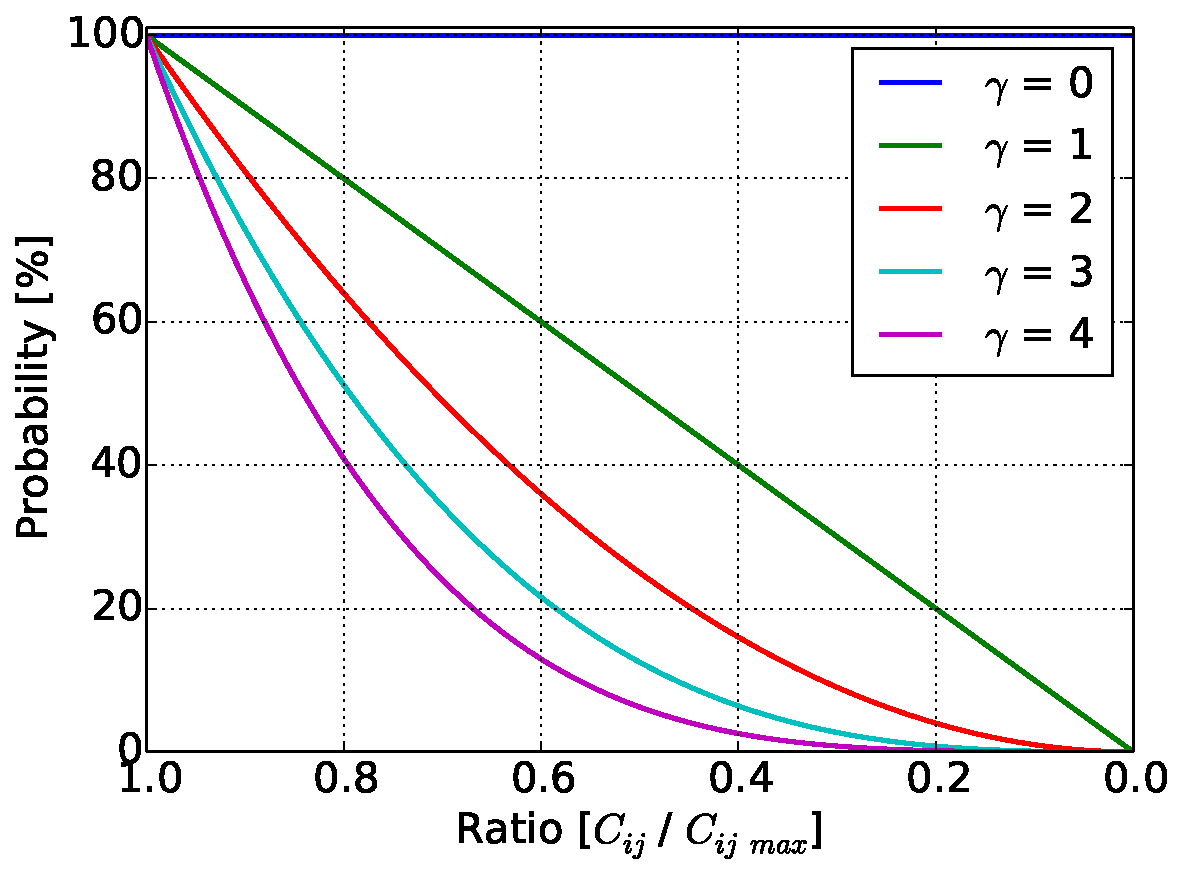
\includegraphics[width=0.7\linewidth]{theory/bilder/interactions}
\caption{Figure shows the probability as a function of their trade ratio.}
\label{fig:interactions}
\end{figure}










\pagebreak
\section{Computational theory}

This project consists of four different cases with a different degree of complexity. For the basis case and the savings case it is enough to use the Monte carlo method. The Monte Carlo method is a method that utilizes the fact that a large number of experiments converges towards the expectation value. When the probability of doing a transaction is added the system utilizes the Metropolis Algorithm is implemented. The system has to do a random choice of acceptance or denial of the trade. This random choice is done with the Random Number Generator. A random number i created between $(0-1)$ If the number is less than the probability term, accept the new state. If the number is greater than the energy change then discard the change. The procedure is outlined in four steps.

\begin{itemize}
	\item Chose two agents at random.
	\item Find the probability of acceptance for this new case 
	\item A RNG is used to chose a number between $(0-1)$. Now if the probability term is less then the RNG number, reject the transaction and discard the trade. If not, accept the trade.
	\item Choose a new random number for how much is traded between the two($\epsilon$). 
	\item Update the system with the transfered money.
\end{itemize}





























\pagebreak
\section{Implementation}


The algorithm was implemented as discussed in section \ref{sec:comp-theory} in the program called main.cpp. main.cpp has some functions for different versions of the stock market. The difference between the versions are how likely it is that two random agents will trade. For more insight see section \ref{sec:phys-theory}.\footnote{All of the programs discussed in this section can be found at \href{https://github.com/erikfsk/Project-5}{\color{blue}{github}}}.
\\
\\
Many different simulations is needed for this report. This is why a parallelized version has been made. MPI is used since it is easy to implement. Most of the code in the parallelized version is the same as for the non-parallelized. The parallelized version should then be X times faster then the normal version with X cores. Each thread and runs the simulations for some given values for $\alpha$, $\lambda$ and $\gamma$. The values is determined by the rank of the thread and will therefor be unique to other thread's values.\footnote{\href{https://www.intel.com/content/www/us/en/architecture-and-technology/hyper-threading/hyper-threading-technology.html}{\color{blue}{Intel Hyper-Threading Technology}}}


\begin{center}
\label{tab:parallell}
\captionof{table}{The agents were given $10^7$ opportunities to do a transaction and the system was simulated 160 times. The test ran on a macbook pro 15. It has a quad core CPU. Expected difference is 4. The difference was higher, then expected. This is due to the Hyper-Threading technology in this CPU. }
\begin{tabularx}{\textwidth}{c X c X c X c X c}
    \hline 
    \hline 
       	Version && Normal && MPI && Expected difference && Actual difference\\ 
    \hline
        A   	&&      35.147  s	&&		7.361 s 	&&	4.000	&&	4.774	\\  
        D   	&&      98.112  s	&&		17.202 s	&&	4.000	&&	5.764	\\
        E   	&&      226.522 s	&&		45.608 s	&&	4.000	&&	4.966	\\
    \hline
\end{tabularx}
\end{center}


\begin{center}
\label{tab:expected-time}
\captionof{table}{
For scaling we expect a time increased proportional to the size increase. The table shows how we expect the time to develop and how it actually it develops. There is a minor difference from expected and calculated and that comes from the fact that the program does more then just the algorithm and the fact that the algorithm has not been perfectly implemented.}
\begin{tabularx}{\textwidth}{c X c X c X c X c}
    \hline 
    \hline 
        Version && \# Simulations&& Expected time && Actual time && $T_{i}$ / $T_{10}$\\ 
    \hline
        A   	&& 10  &&      x		&&		2.252 s 	&&	1.000	\\  
        A   	&& 160 &&      16x		&&		35.147 s	&&	15.60	\\
        D   	&& 10  &&      x		&&		6.229 s 	&&	1.000	\\  
        D   	&& 160 &&      16x		&&		98.112 s	&&	15.75	\\
        E   	&& 10  &&      x		&&		12.876 s 	&&	1.000	\\  
        E   	&& 160 &&      16x		&&		226.522 s	&&	17.59	\\
    \hline
\end{tabularx}
\end{center}



\begin{figure}[H]
    \centering
    \begin{subfigure}{0.19\textwidth}
        \centering
        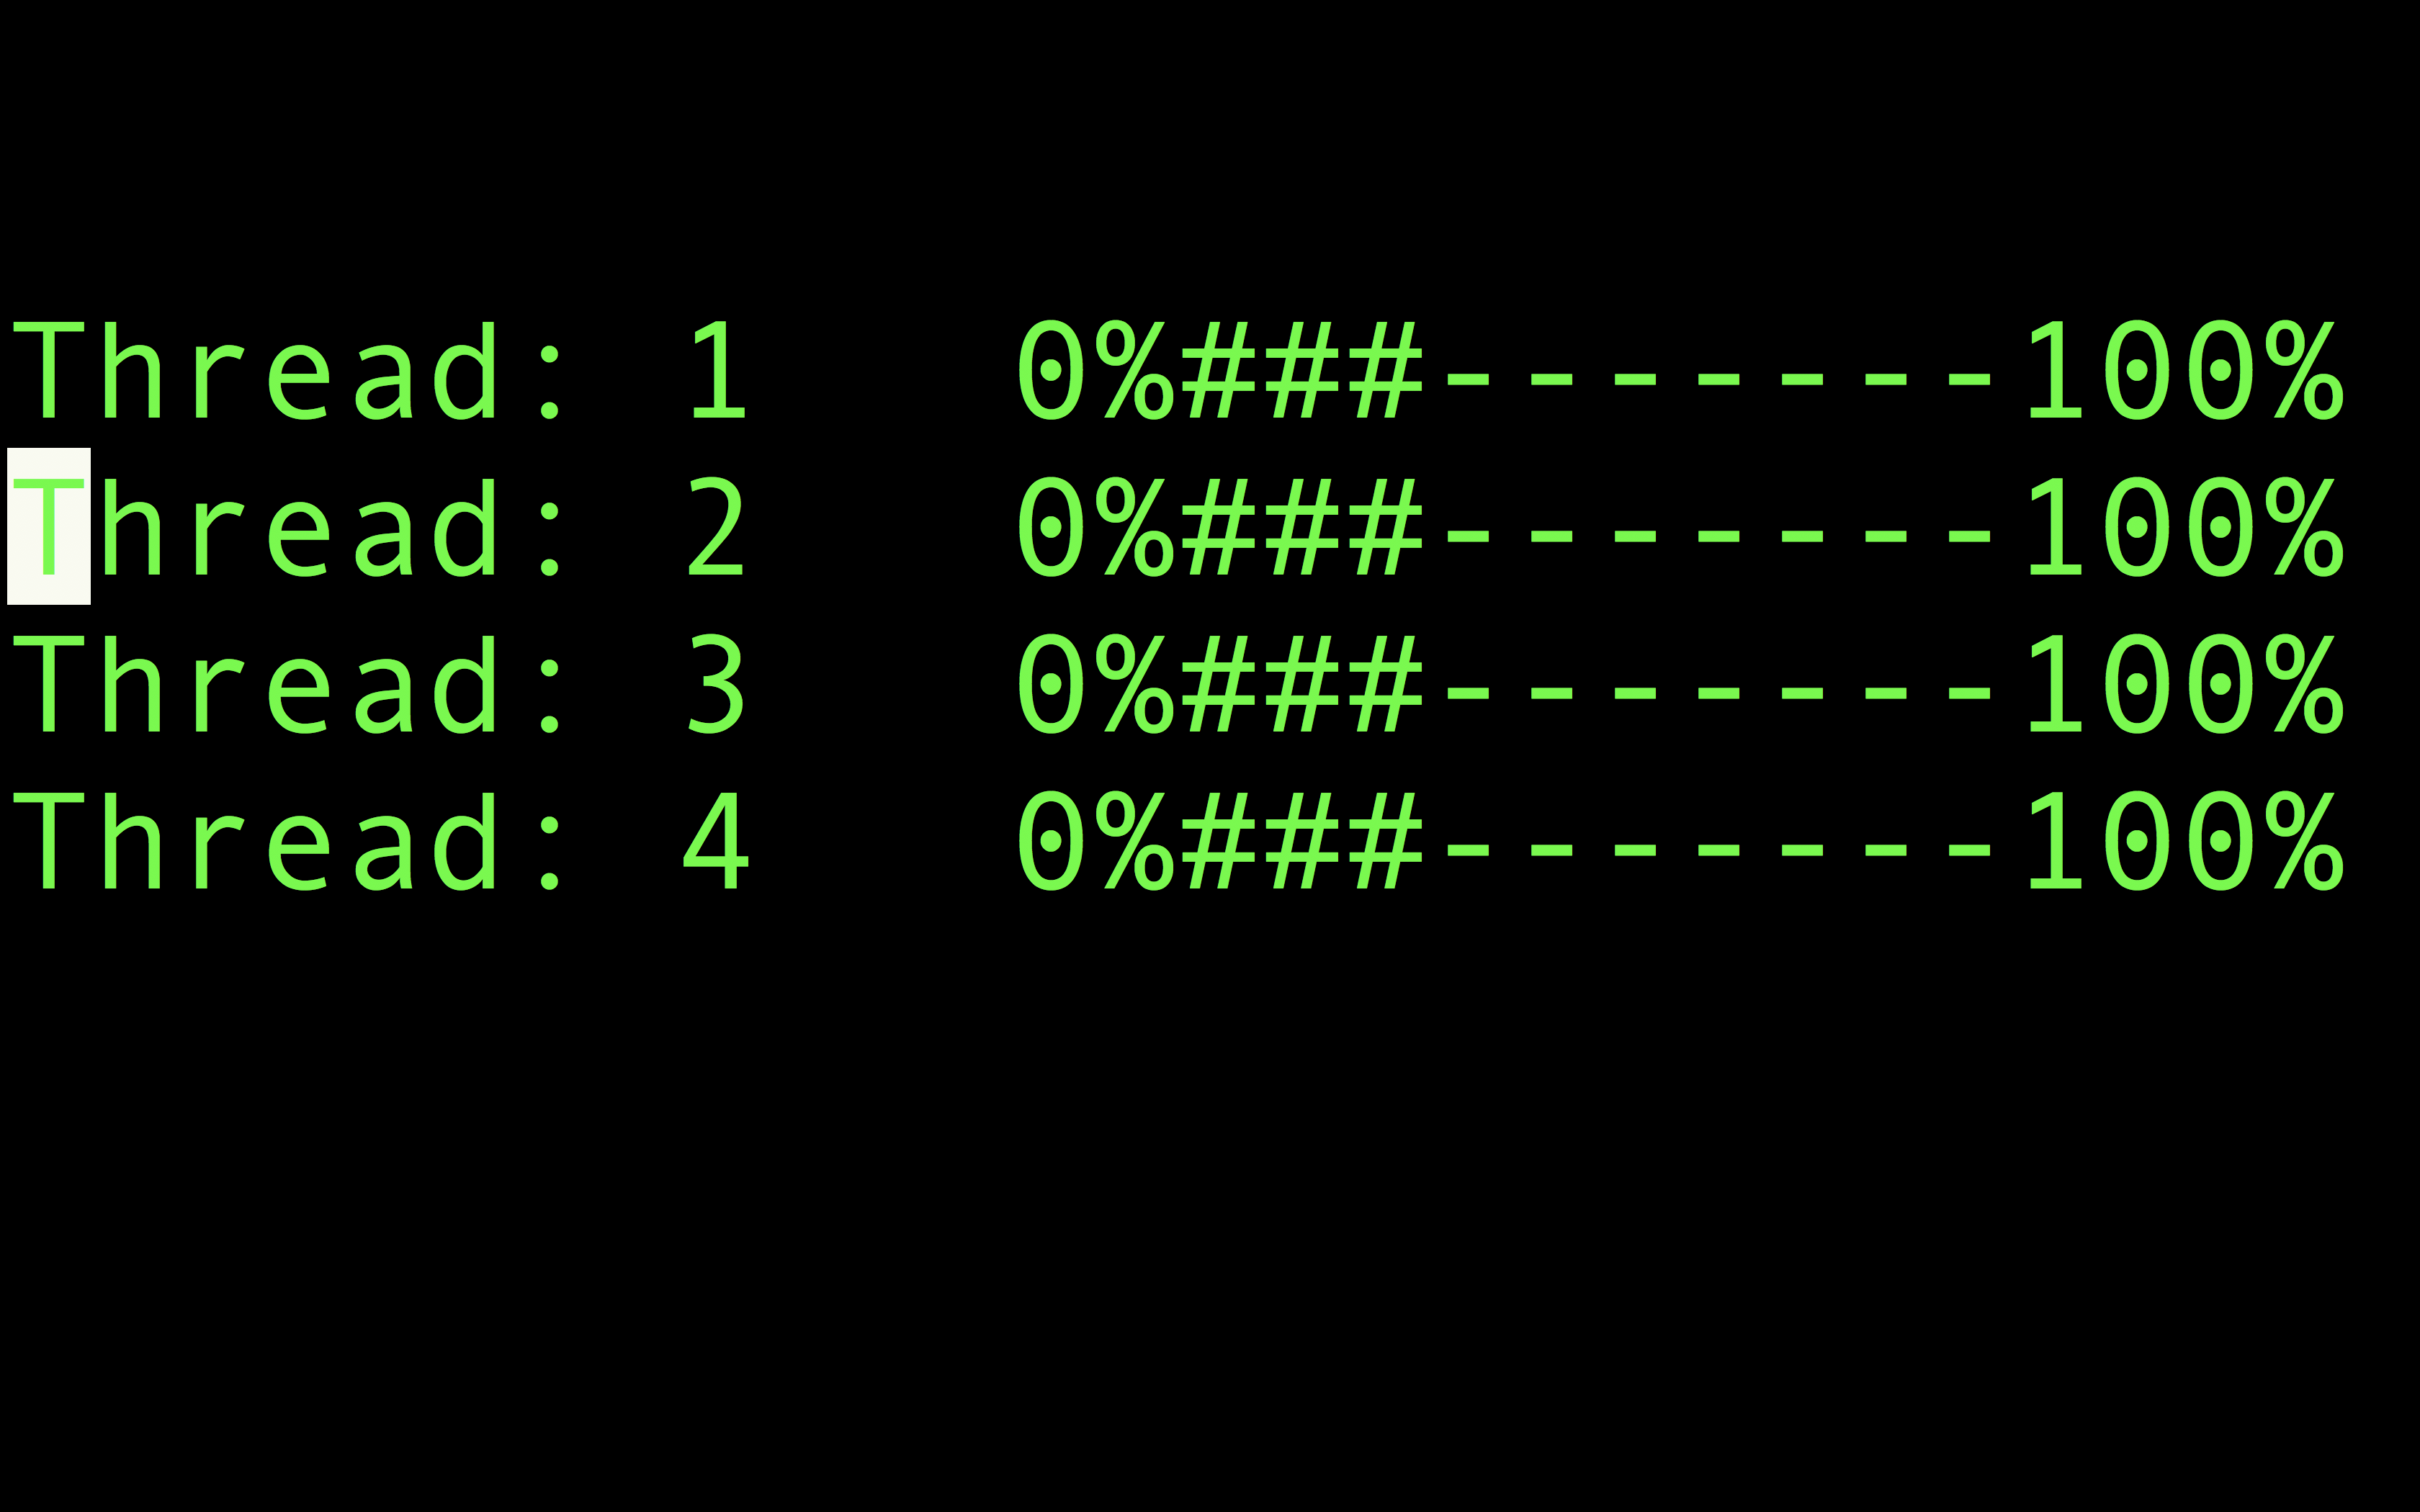
\includegraphics[width=1.11\linewidth]{method/bilder/2}
    \end{subfigure}
    ~ 
    \begin{subfigure}{0.19\textwidth}
        \centering
        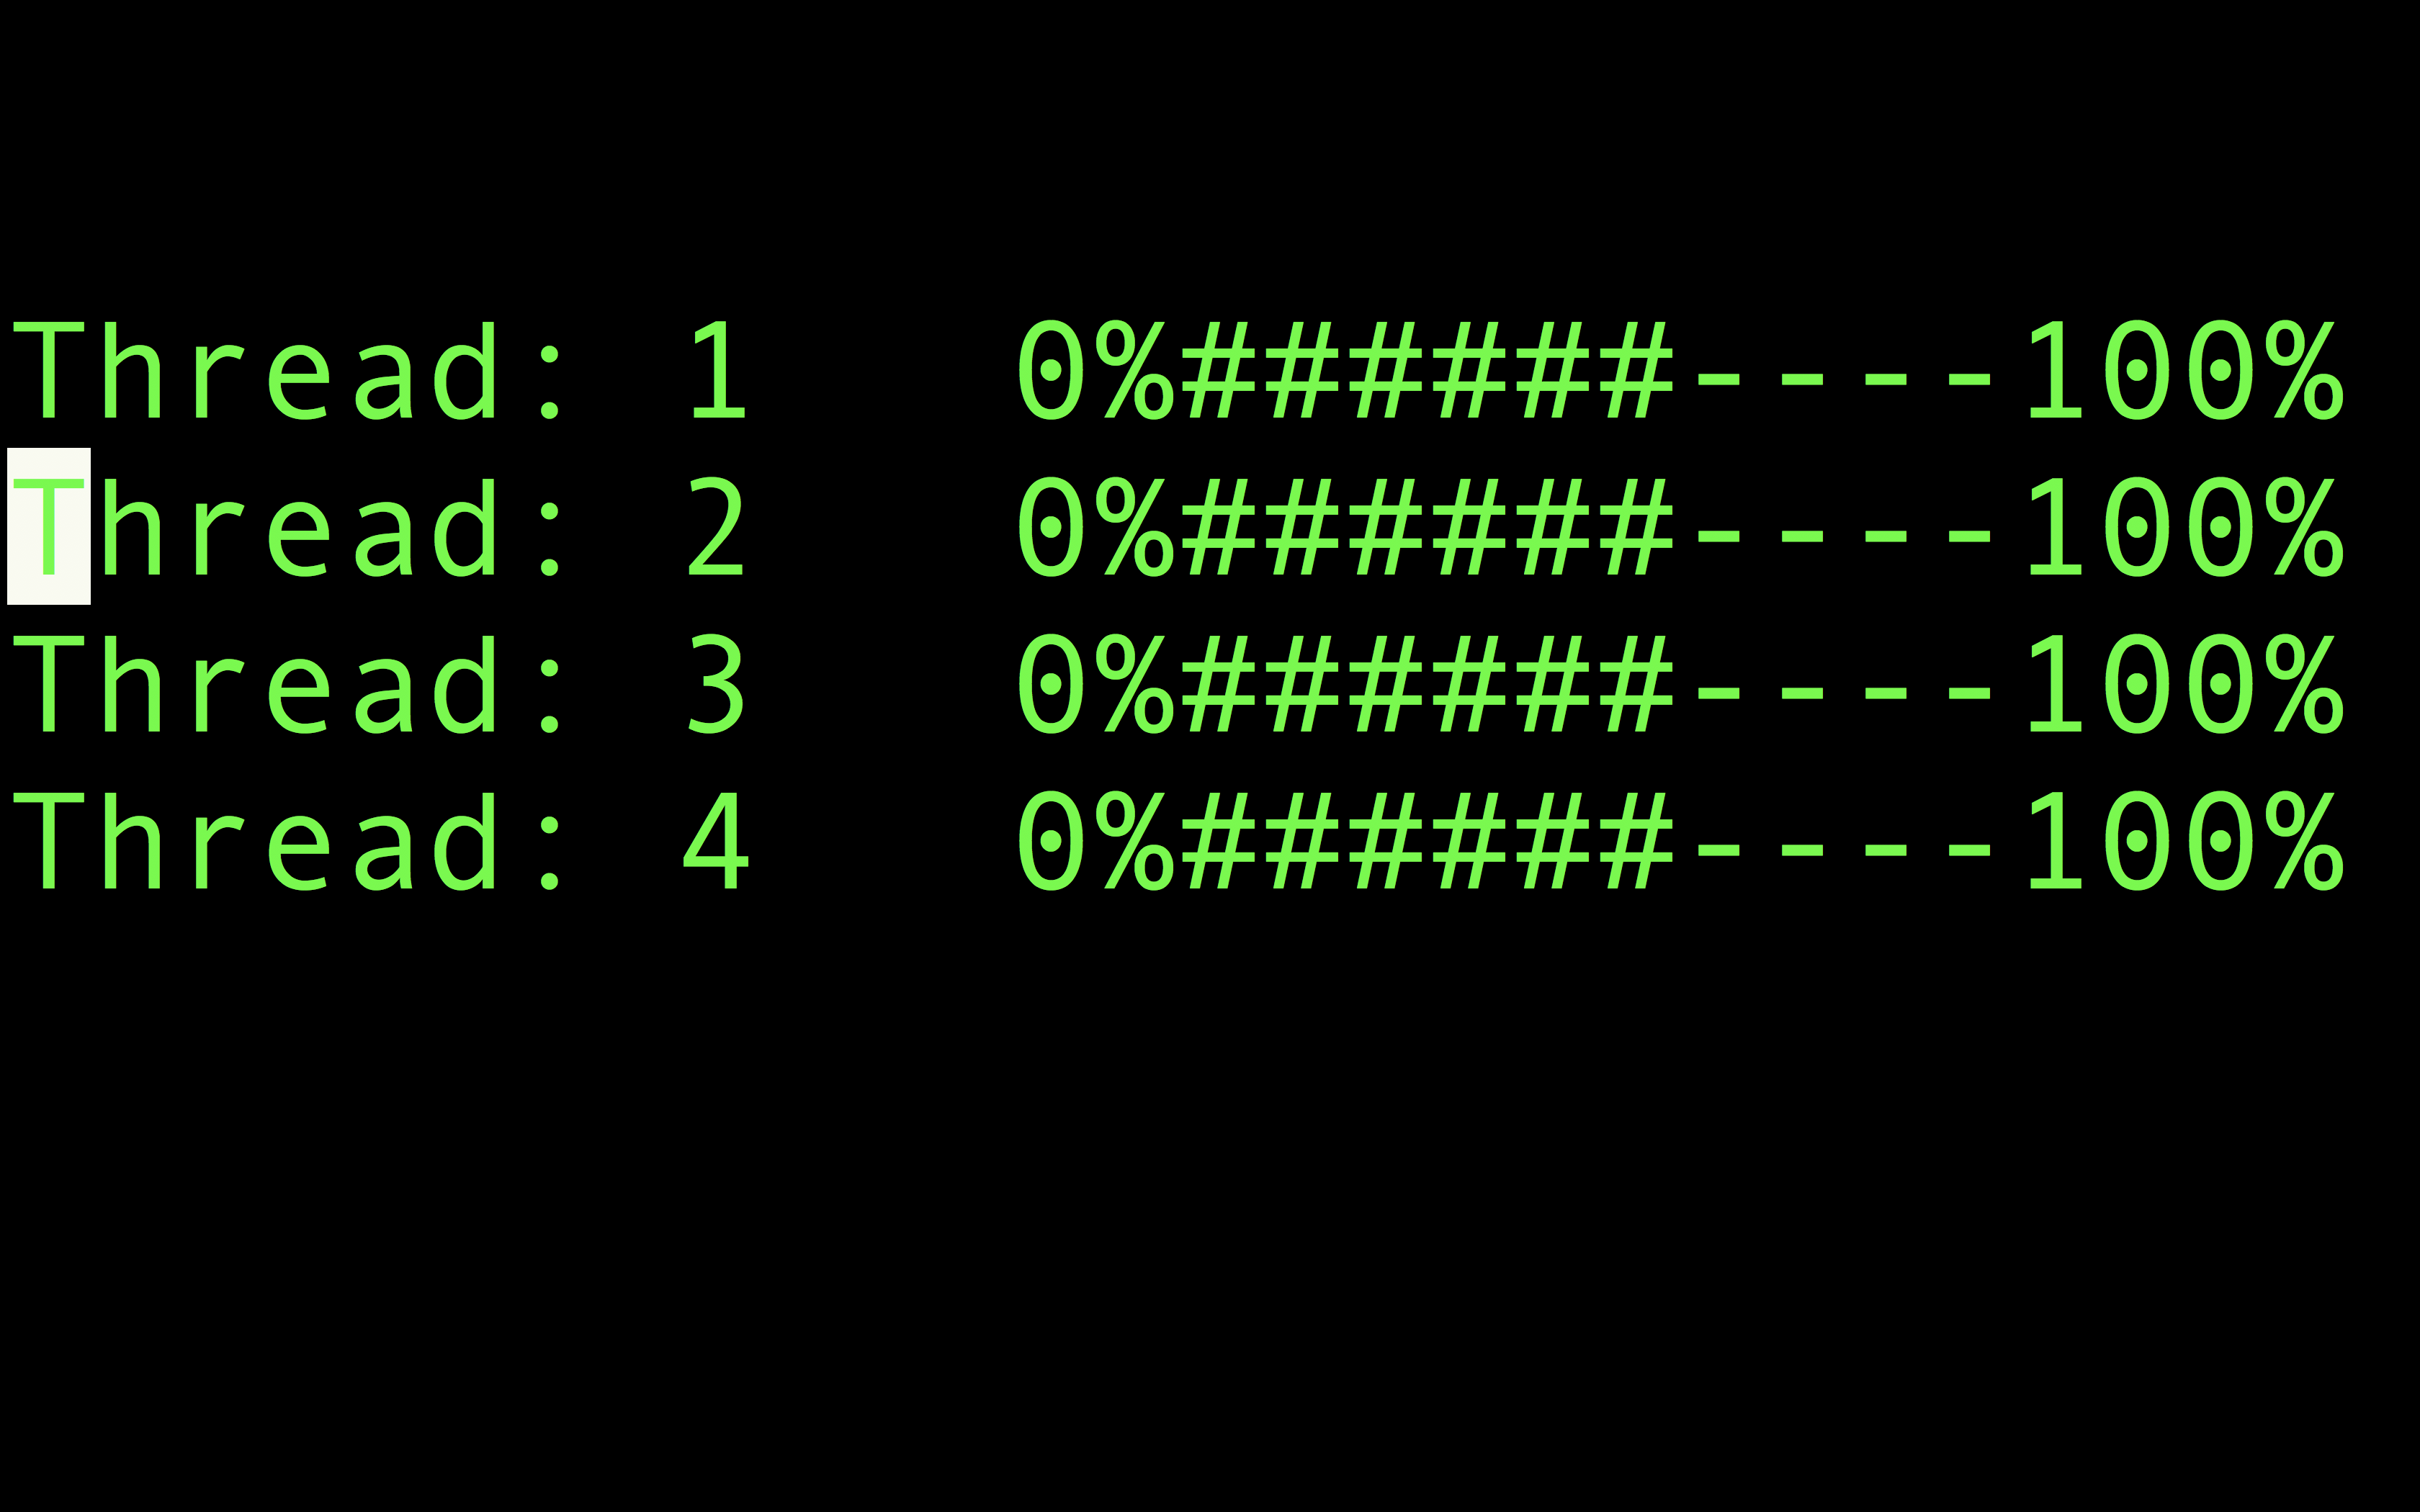
\includegraphics[width=1.11\linewidth]{method/bilder/3}
    \end{subfigure}
    ~ 
    \begin{subfigure}{0.19\textwidth}
        \centering
        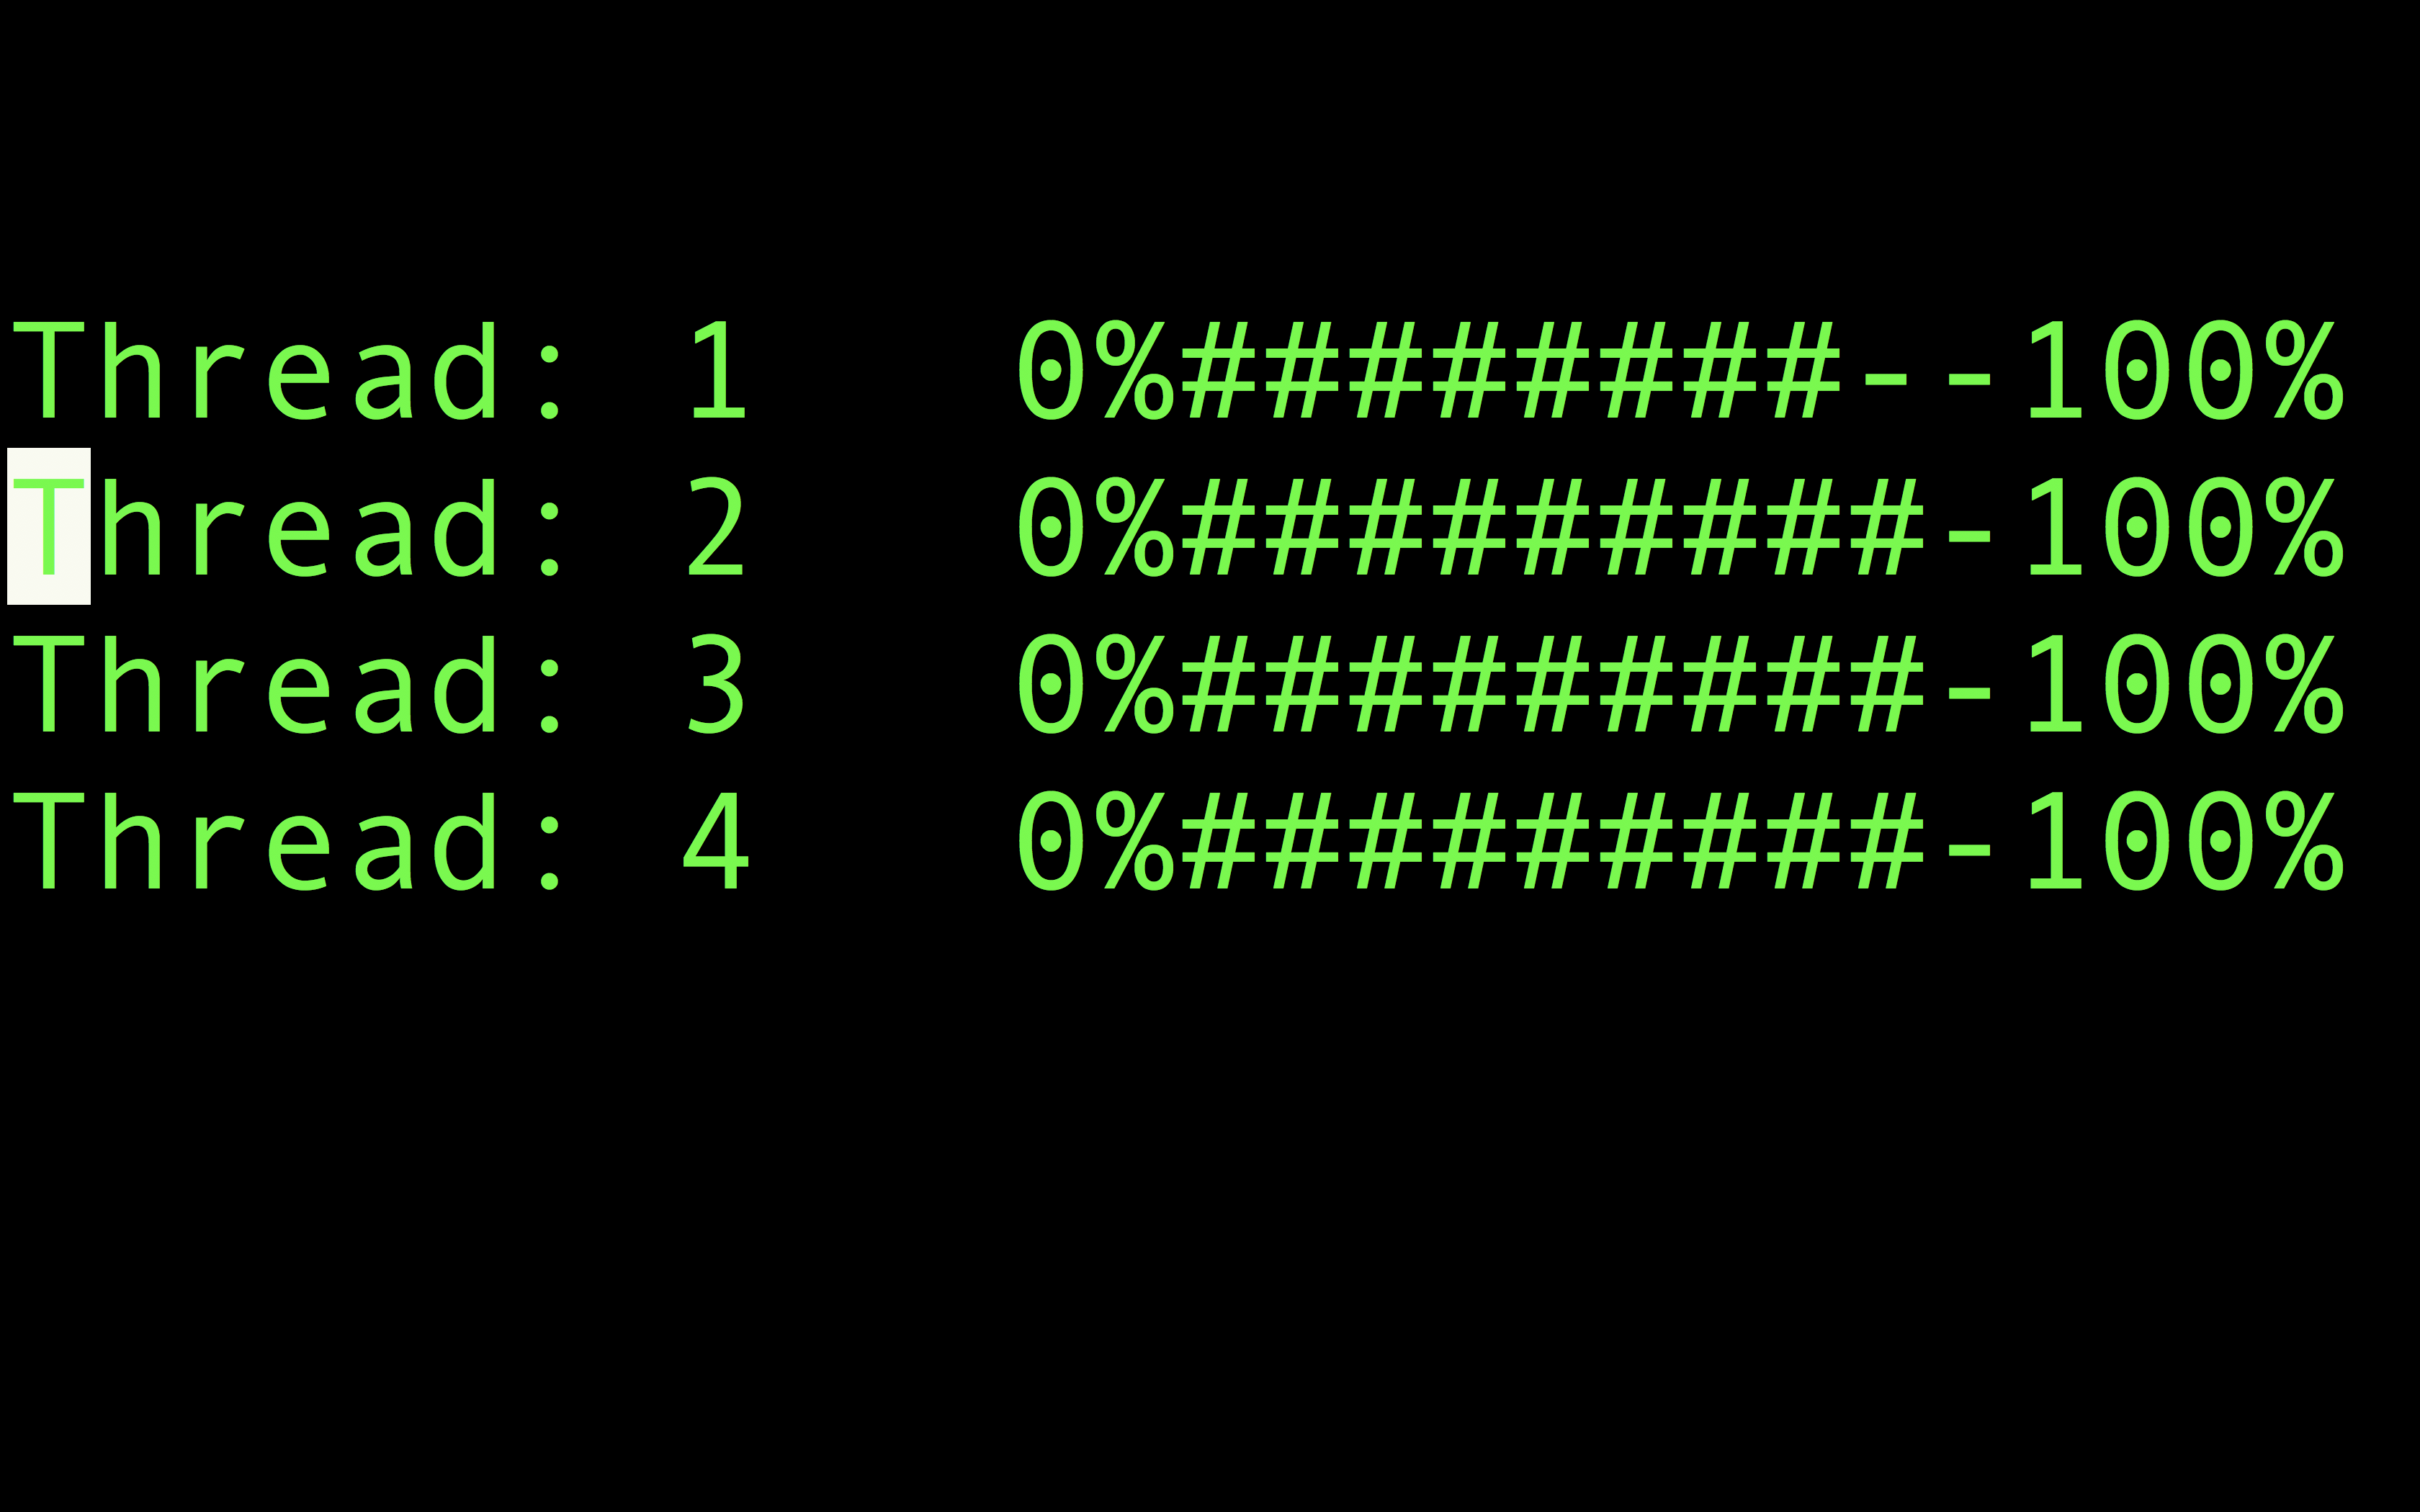
\includegraphics[width=1.11\linewidth]{method/bilder/4}
    \end{subfigure}
    ~ 
    \begin{subfigure}{0.19\textwidth}
        \centering
        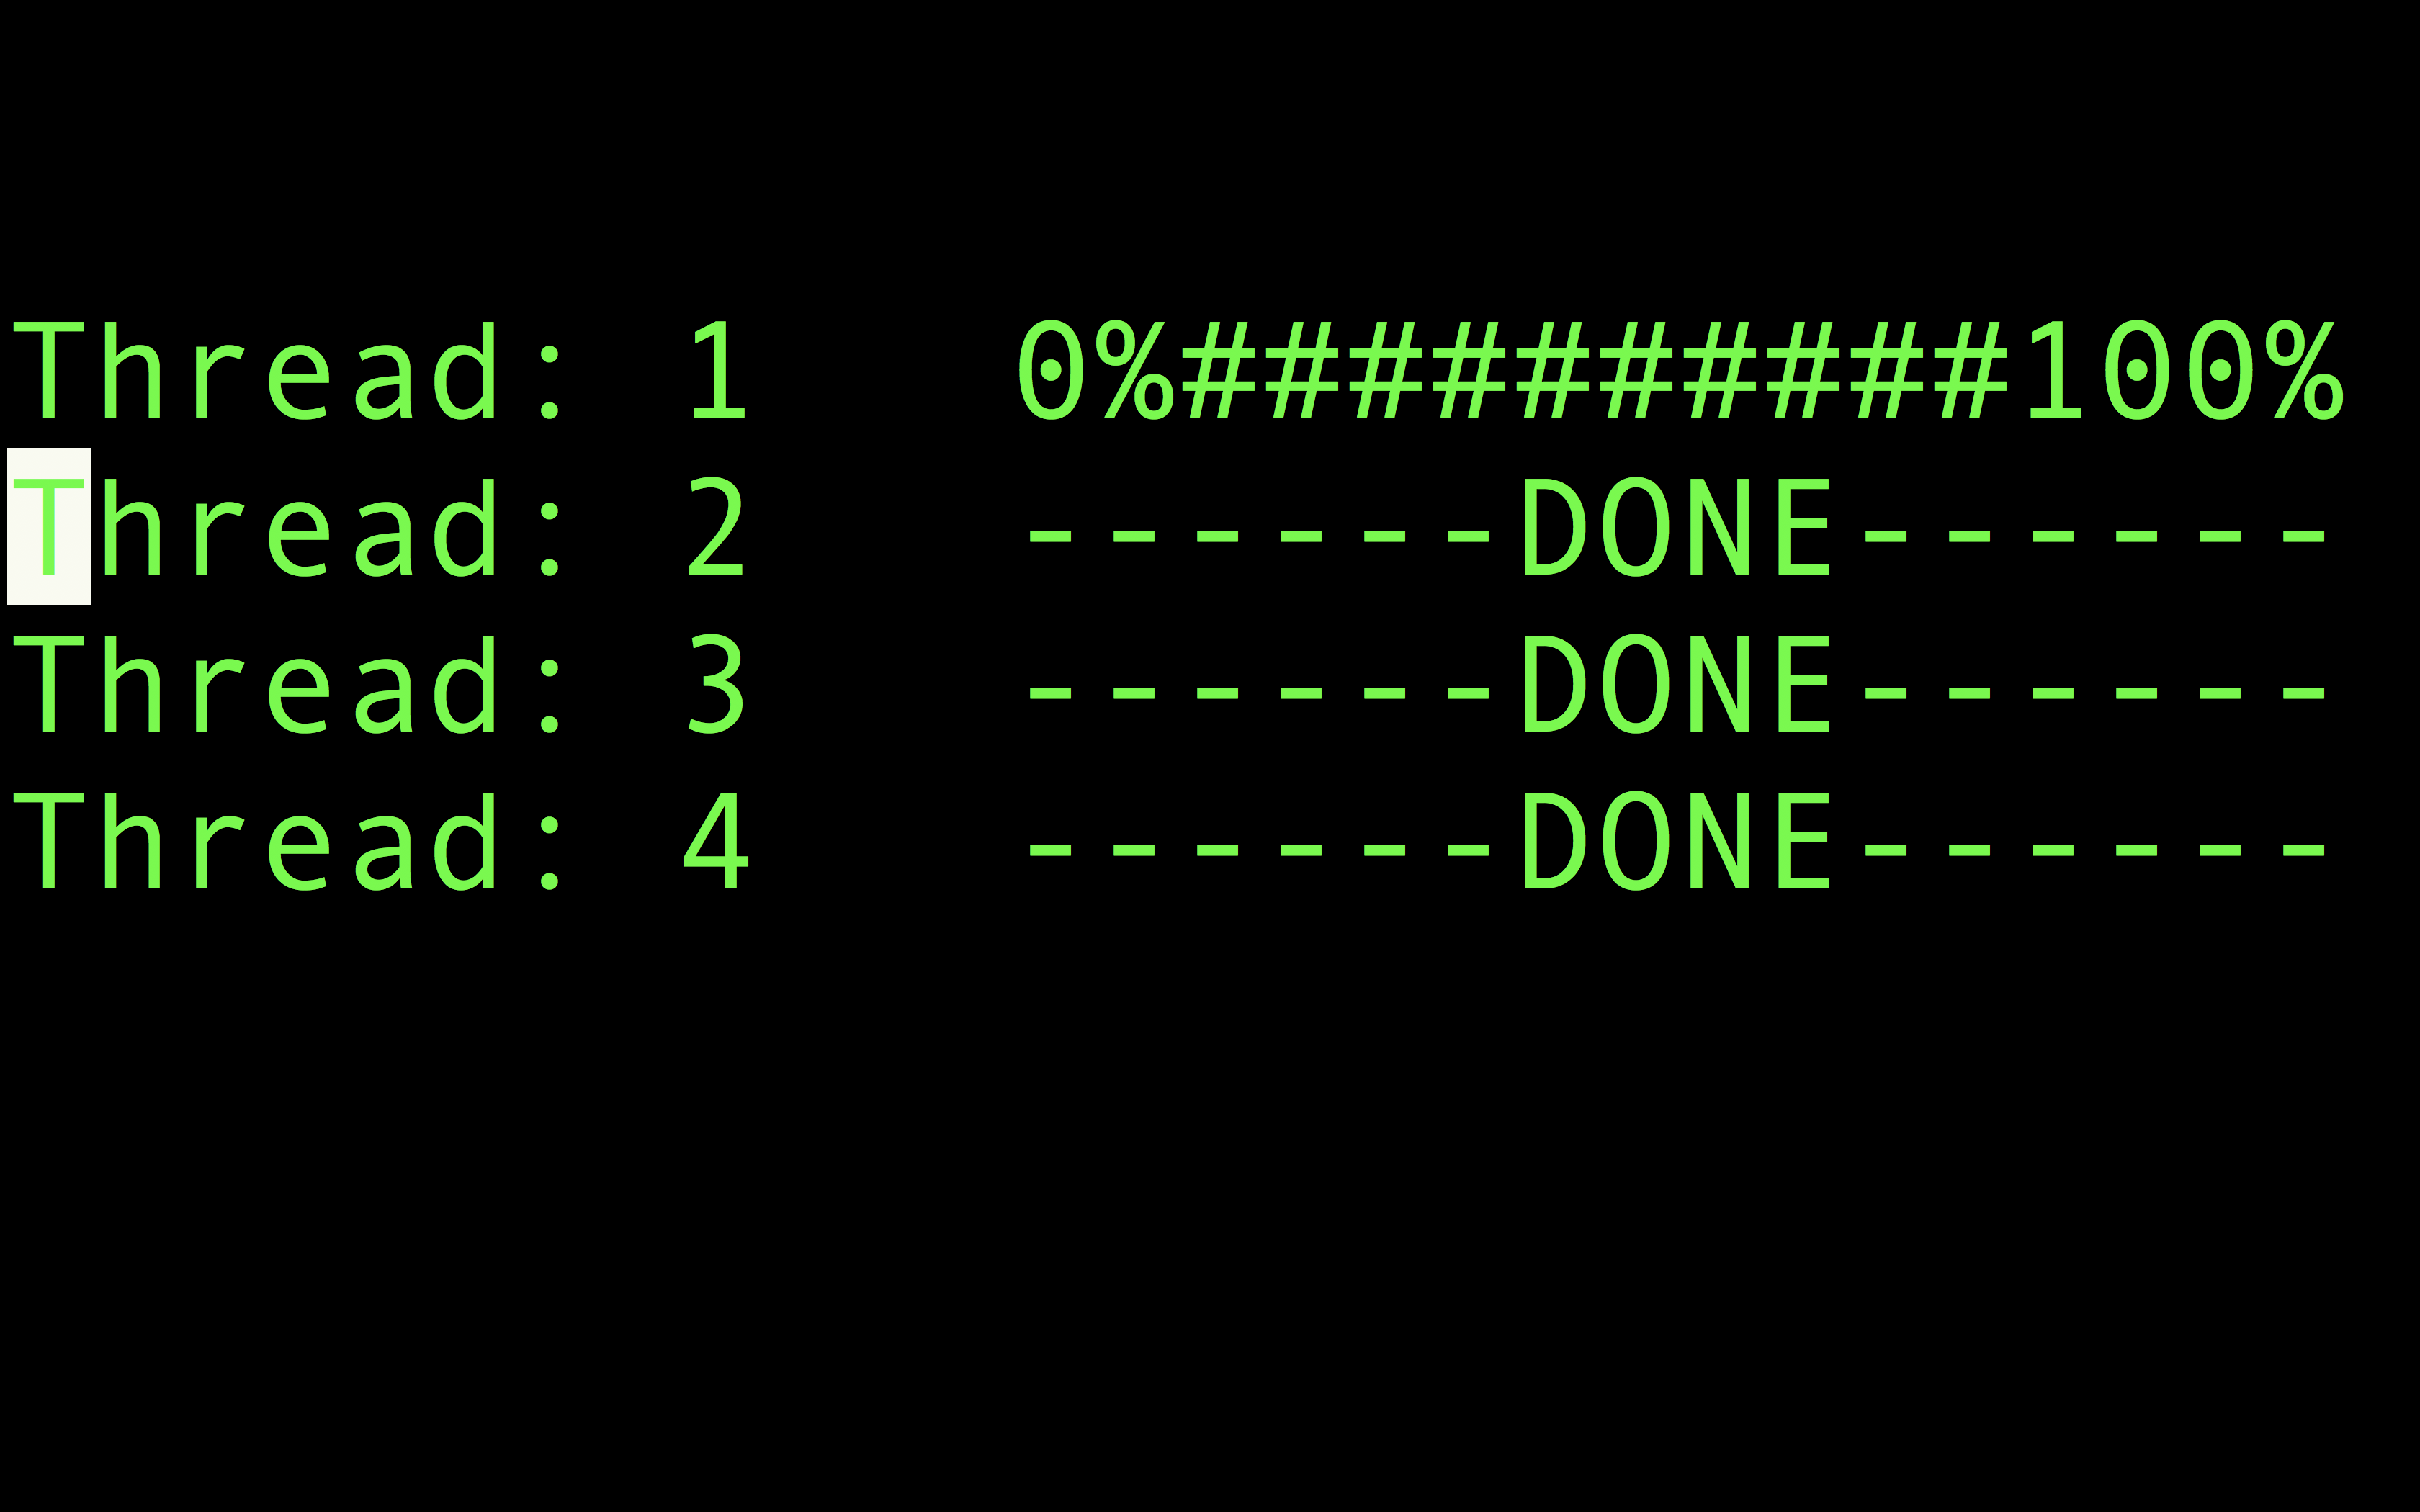
\includegraphics[width=1.11\linewidth]{method/bilder/5}
    \end{subfigure}
    \caption{A progress bar was made for the program. It shows the progress for each individual thread. The progress bar works for 1 to 4 threads. More then 4 threads might look funny. By the way, we are A students in the newly announced PRO101 subject. }
    \label{fig:progress}
\end{figure}


\footnote{
    \href
    {https://shortridgedailyecho.org/wp-content/uploads/2017/08/definition-procrastination.png}
    {
    \color{blue}{PRO101: Procrastination for students}
    }
    }
% \animategraphics{12}{gif-}{1}{32}

\pagebreak
\section{Result \& Discussion}
\pagebreak
\subsection{5a \& 5b}
\begin{figure}[H]
    \centering
    \begin{subfigure}{0.5\textwidth}
        \centering
        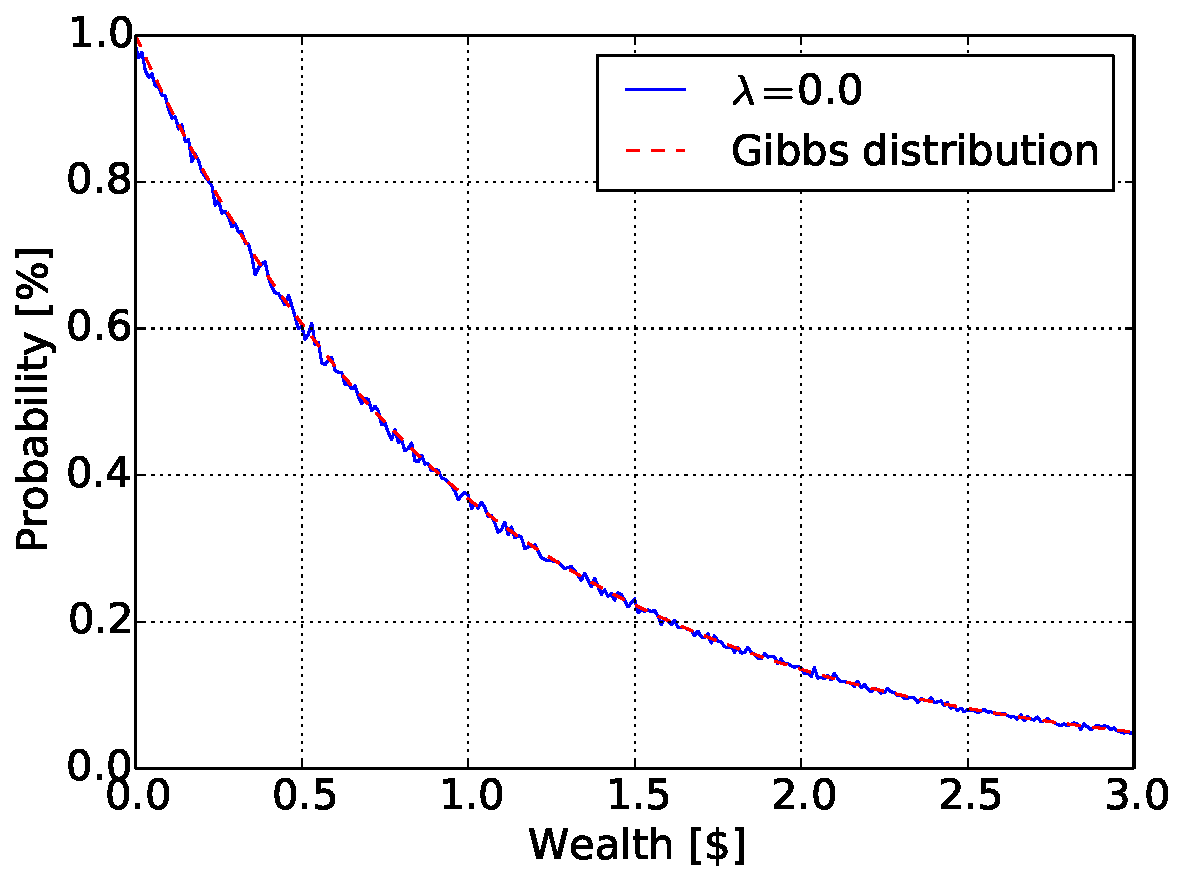
\includegraphics[width=\linewidth]{result/bilder/5a-correct}
        \caption{}
    \end{subfigure}%
    ~ 
    \begin{subfigure}{0.5\textwidth}
        \centering
        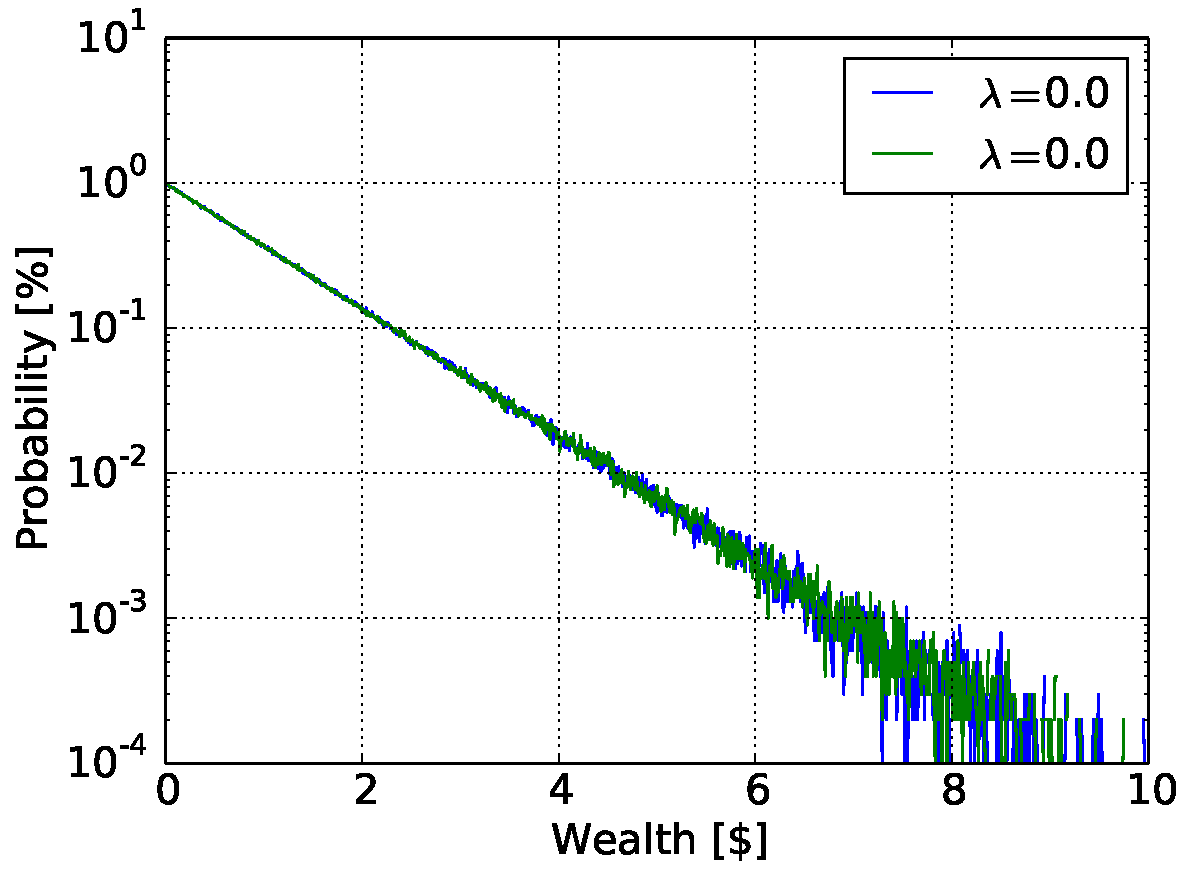
\includegraphics[width=\linewidth]{result/bilder/5b-correct}
        \caption{}
    \end{subfigure}
    \caption{a) Shows how E behaves around $T_C$ b) Shows how |M| develops near $T_C$.}
    \label{fig:5a-b}
\end{figure}




























\pagebreak
\subsection{5c}
\begin{figure}[H]
    \centering
    \begin{subfigure}{0.5\textwidth}
        \centering
        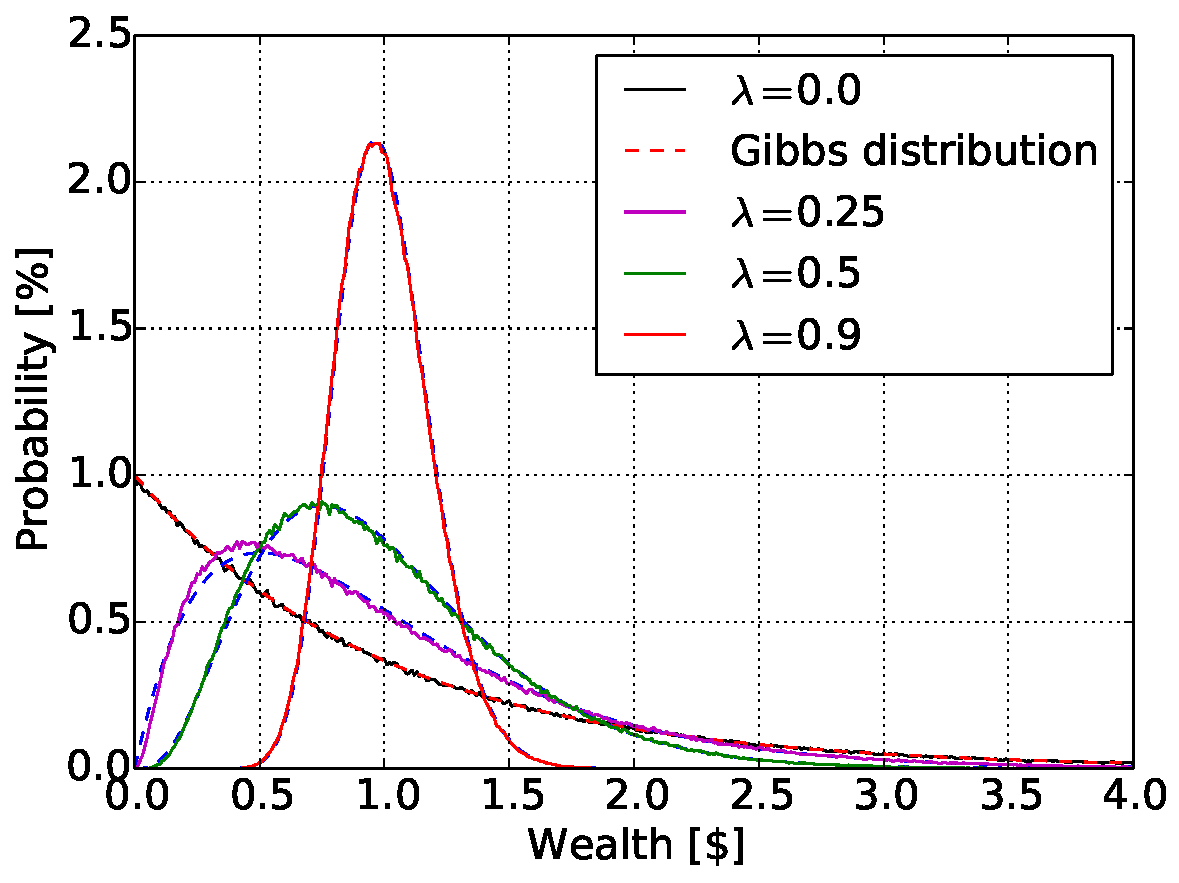
\includegraphics[width=\linewidth]{result/bilder/5c}
        \caption{}
    \end{subfigure}%
    ~ 
    \begin{subfigure}{0.5\textwidth}
        \centering
        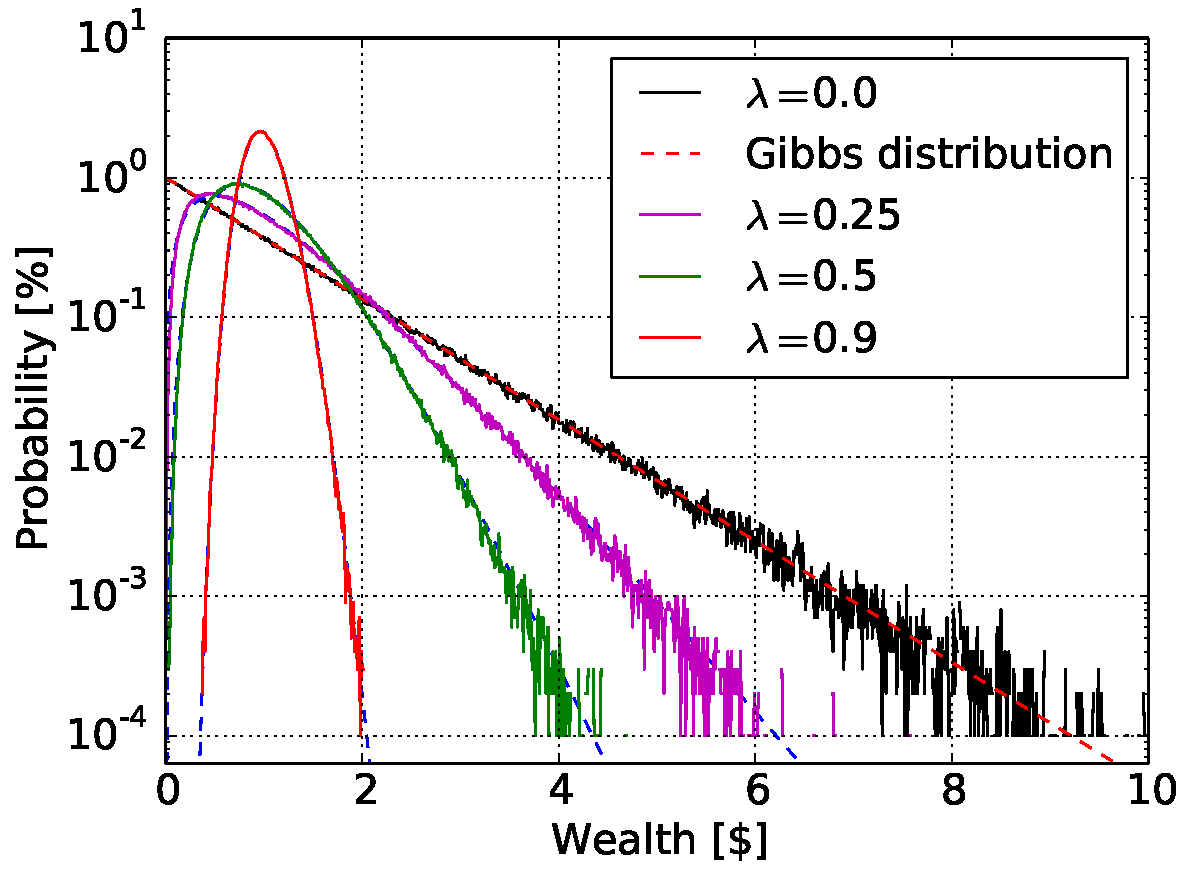
\includegraphics[width=\linewidth]{result/bilder/5c-log}
        \caption{}
    \end{subfigure}
    \caption{a) Shows how E behaves around $T_C$ b) Shows how |M| develops near $T_C$.}
    \label{fig:5c}
\end{figure}




























\pagebreak
\subsection{5d}
\begin{figure}[H]
    \centering
    \begin{subfigure}{0.5\textwidth}
        \centering
        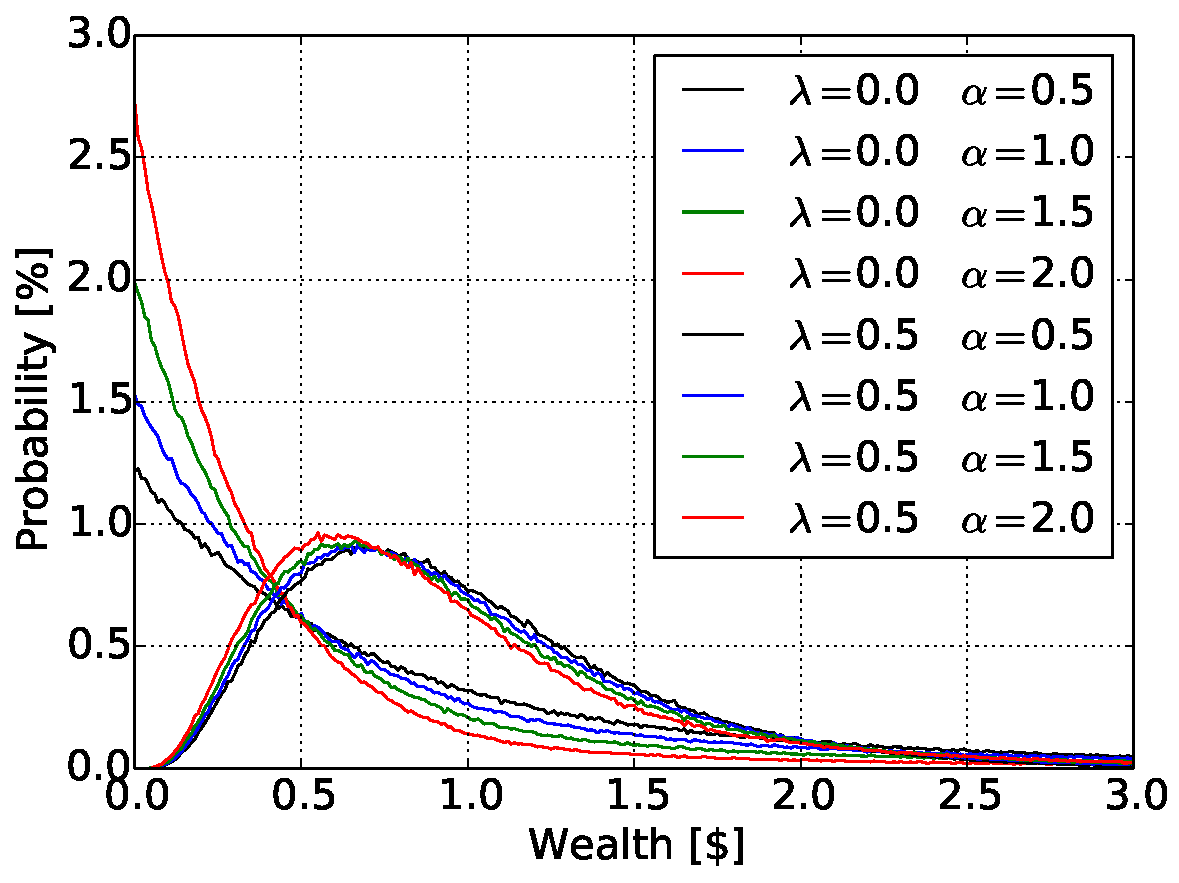
\includegraphics[width=\linewidth]{result/bilder/5d-0050}
        \caption{}
    \end{subfigure}%
    ~ 
    \begin{subfigure}{0.5\textwidth}
        \centering
        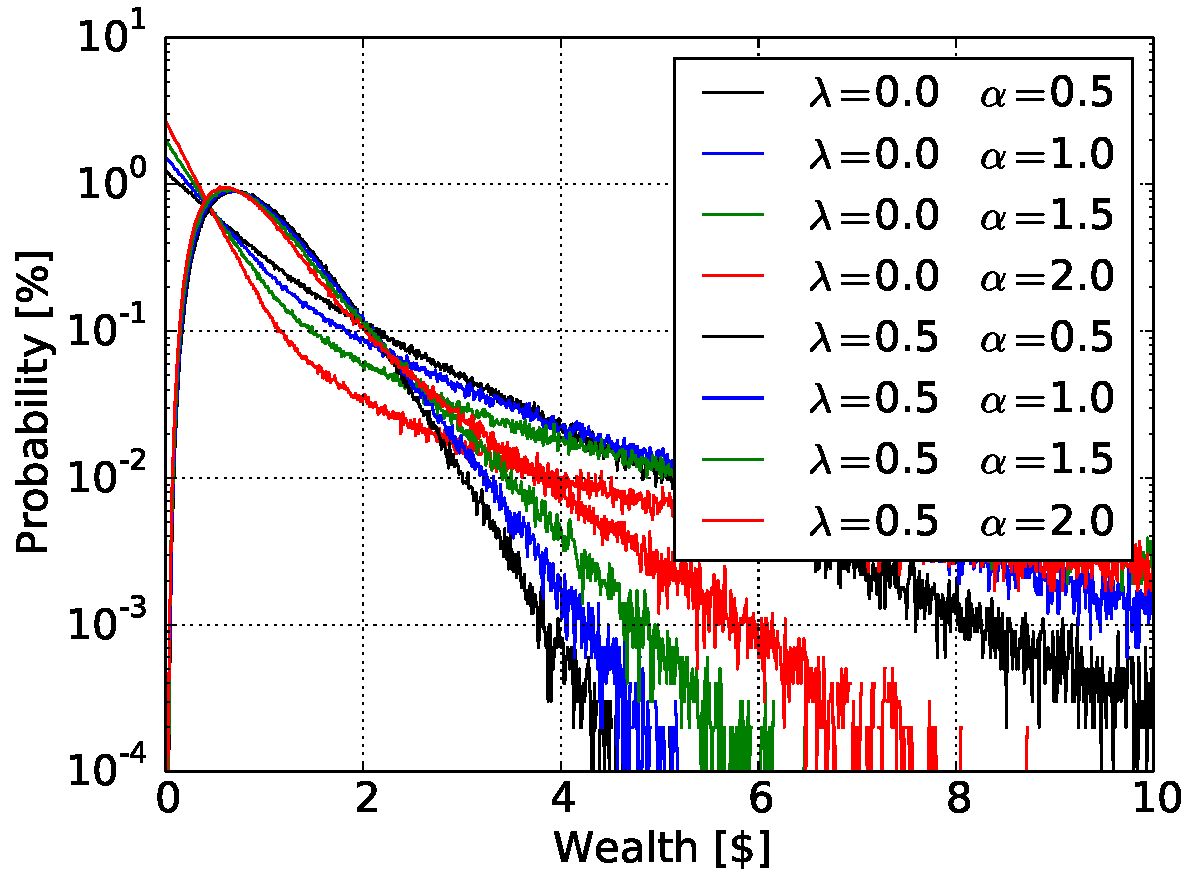
\includegraphics[width=\linewidth]{result/bilder/5d-0050-log}
        \caption{}
    \end{subfigure}
    \caption{a) Shows how E behaves around $T_C$ b) Shows how |M| develops near $T_C$.}
    \label{fig:5d-0050}
\end{figure}



\begin{figure}[H]
    \centering
    \begin{subfigure}{0.5\textwidth}
        \centering
        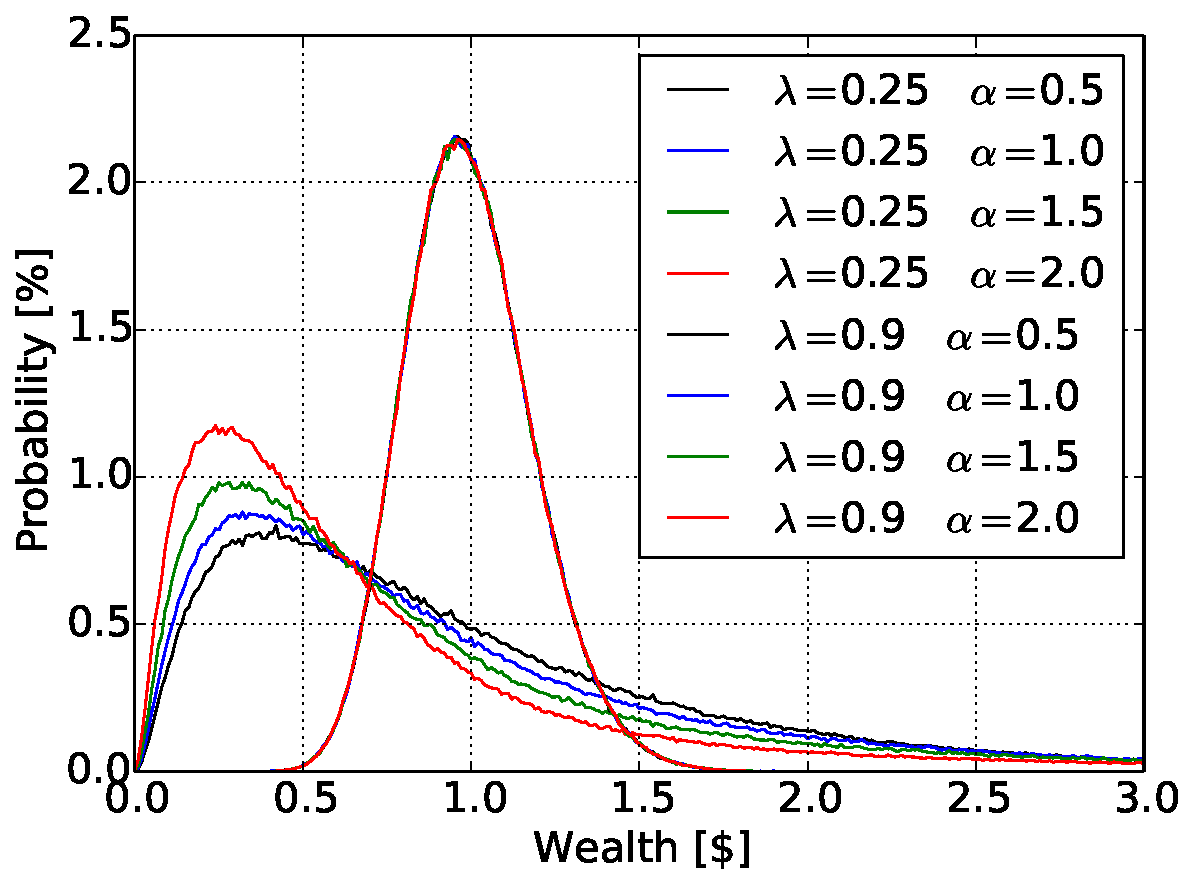
\includegraphics[width=\linewidth]{result/bilder/5d-2590}
        \caption{}
    \end{subfigure}%
    ~ 
    \begin{subfigure}{0.5\textwidth}
        \centering
        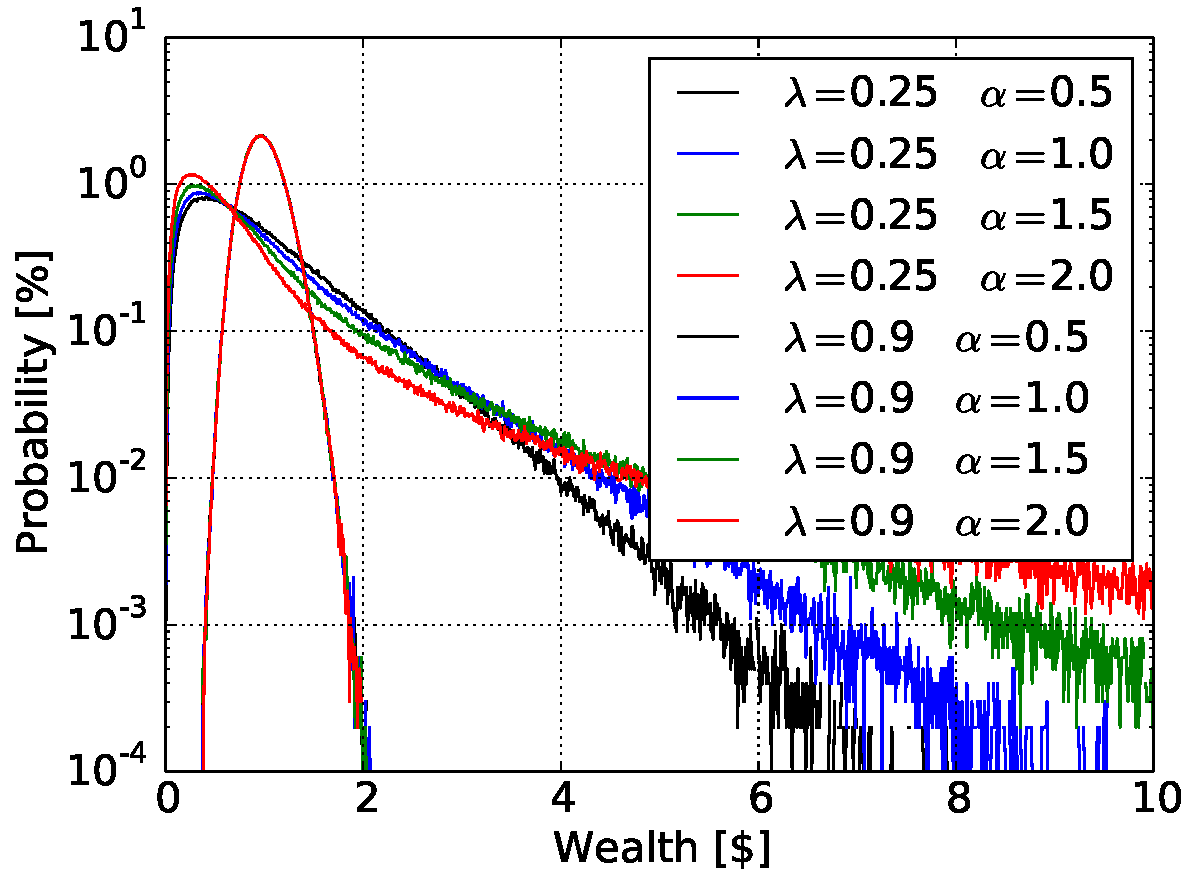
\includegraphics[width=\linewidth]{result/bilder/5d-2590-log}
        \caption{}
    \end{subfigure}
    \caption{a) Shows how E behaves around $T_C$ b) Shows how |M| develops near $T_C$.}
    \label{fig:5d-2590}
\end{figure}



\begin{figure}[H]
    \centering
    \begin{subfigure}{0.5\textwidth}
        \centering
        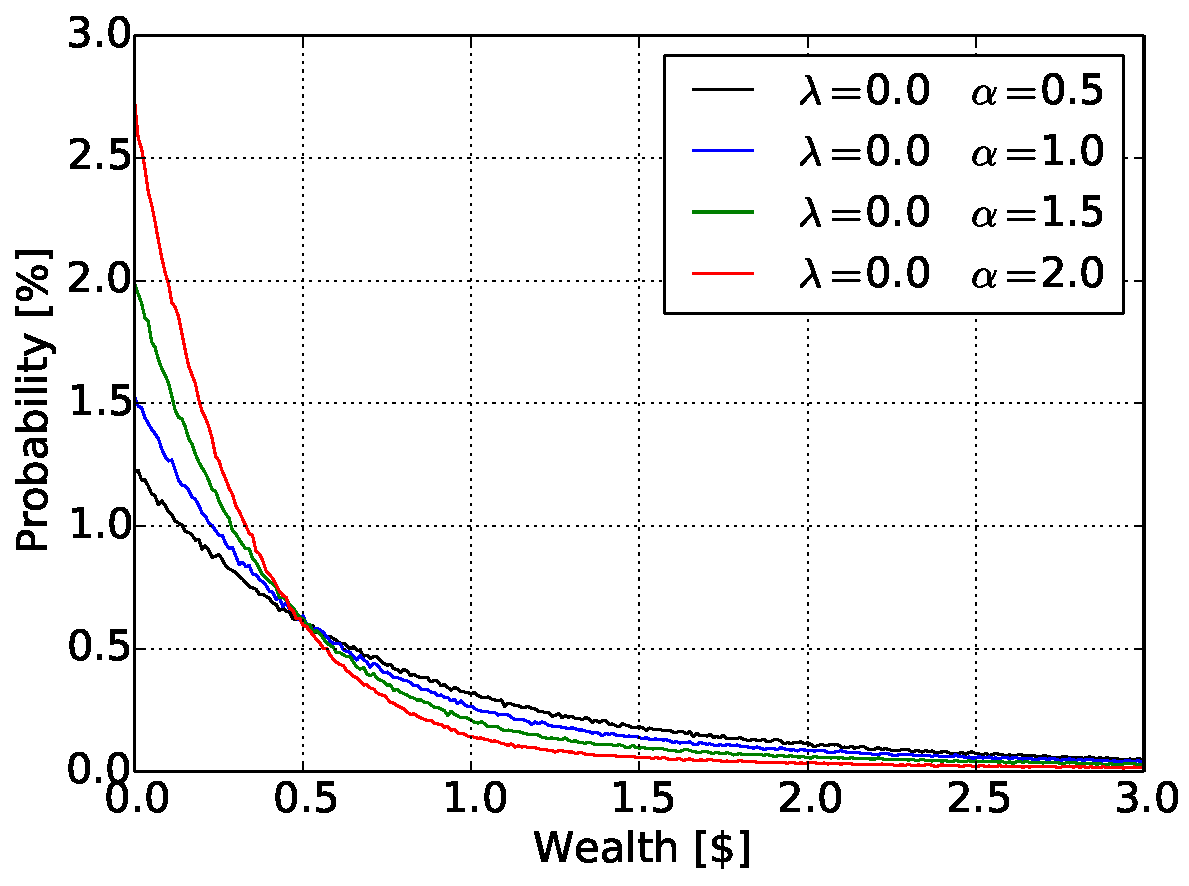
\includegraphics[width=\linewidth]{result/bilder/5d-00}
        \caption{}
    \end{subfigure}%
    ~ 
    \begin{subfigure}{0.5\textwidth}
        \centering
        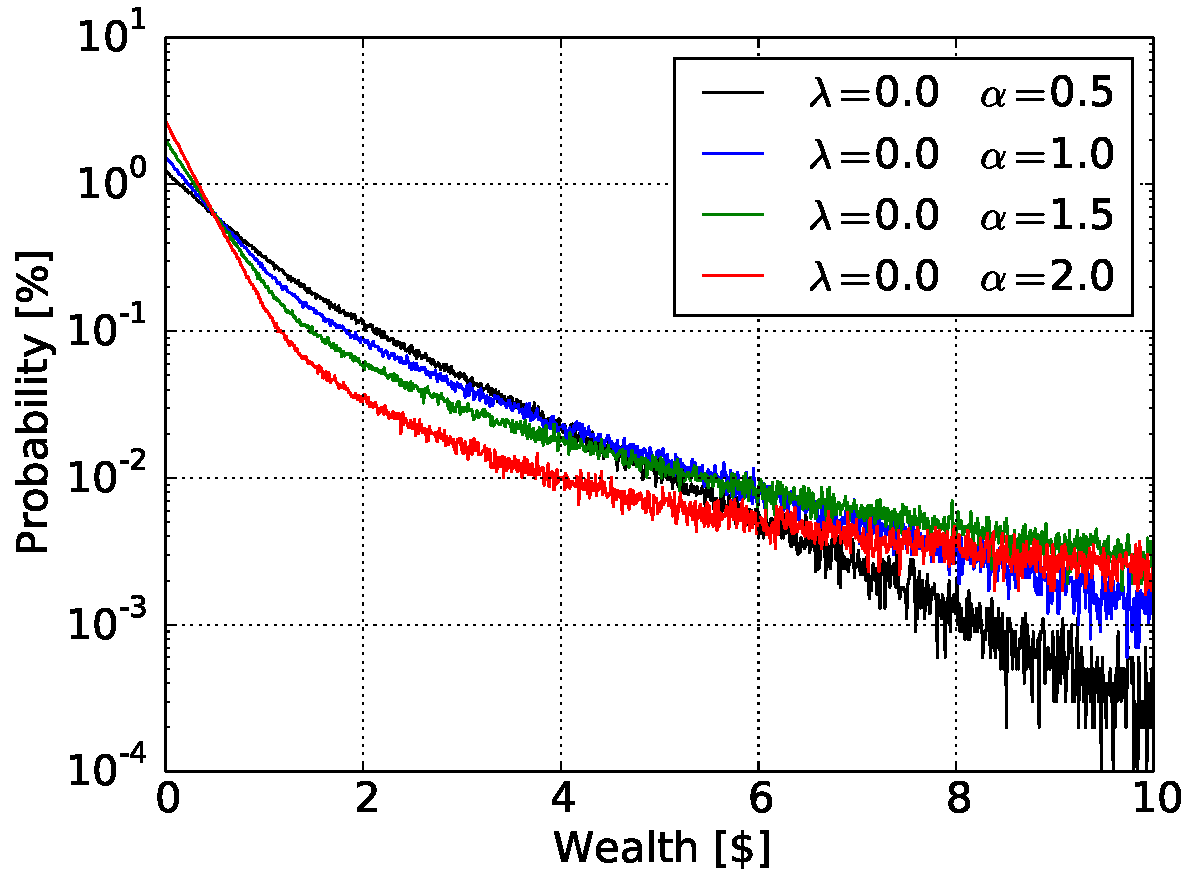
\includegraphics[width=\linewidth]{result/bilder/5d-00-log}
        \caption{}
    \end{subfigure}
    \caption{a) Shows how E behaves around $T_C$ b) Shows how |M| develops near $T_C$.}
    \label{fig:5d-00}
\end{figure}



\begin{figure}[H]
    \centering
    \begin{subfigure}{0.5\textwidth}
        \centering
        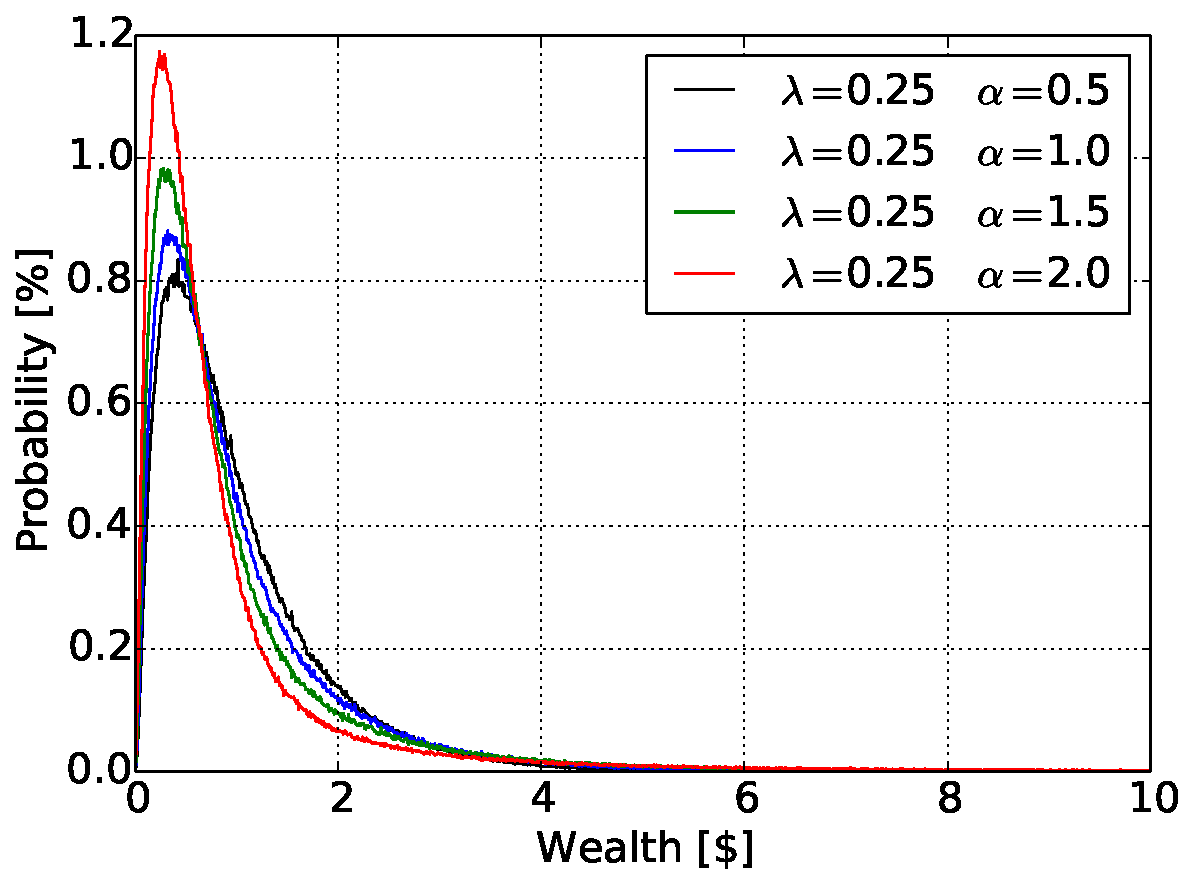
\includegraphics[width=\linewidth]{result/bilder/5d-25}
        \caption{}
    \end{subfigure}%
    ~ 
    \begin{subfigure}{0.5\textwidth}
        \centering
        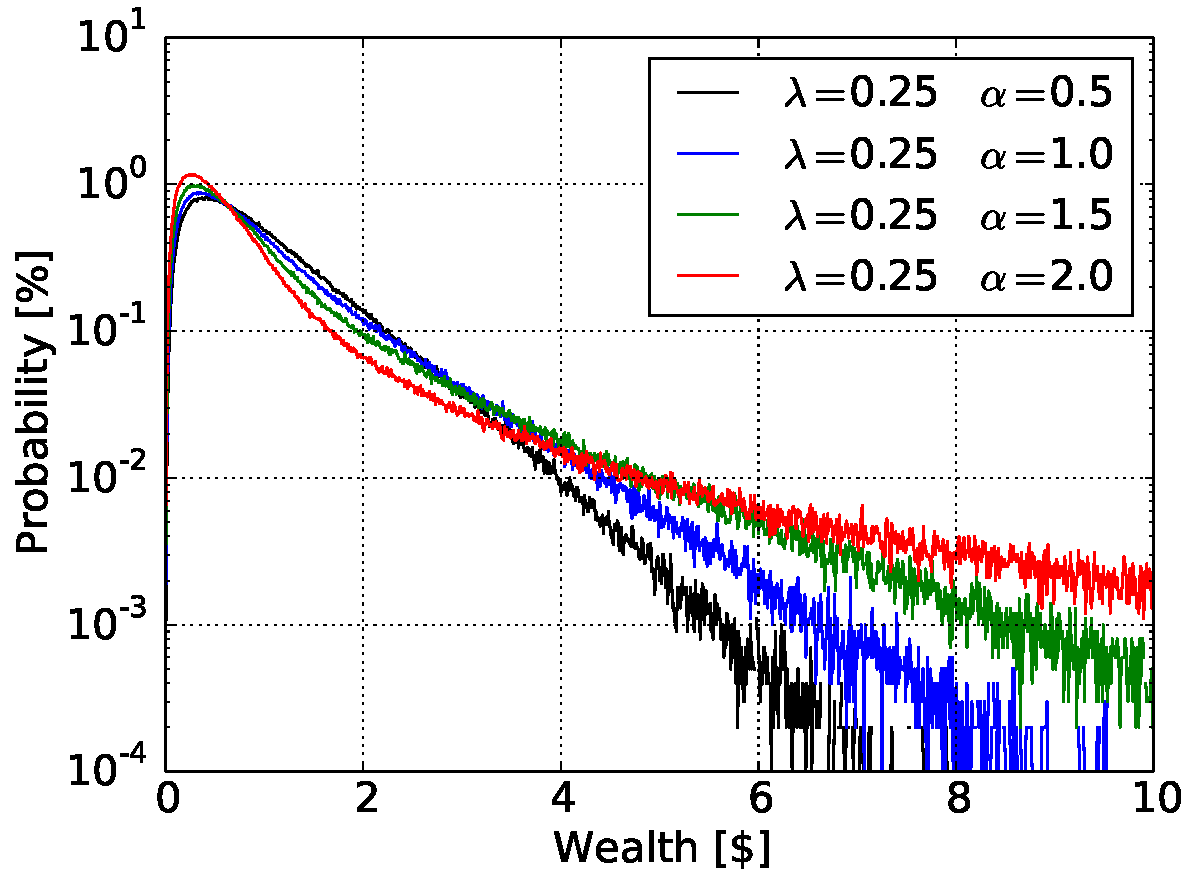
\includegraphics[width=\linewidth]{result/bilder/5d-25-log}
        \caption{}
    \end{subfigure}
    \caption{a) Shows how E behaves around $T_C$ b) Shows how |M| develops near $T_C$.}
    \label{fig:5d-25}
\end{figure}




\begin{figure}[H]
    \centering
    \begin{subfigure}{0.5\textwidth}
        \centering
        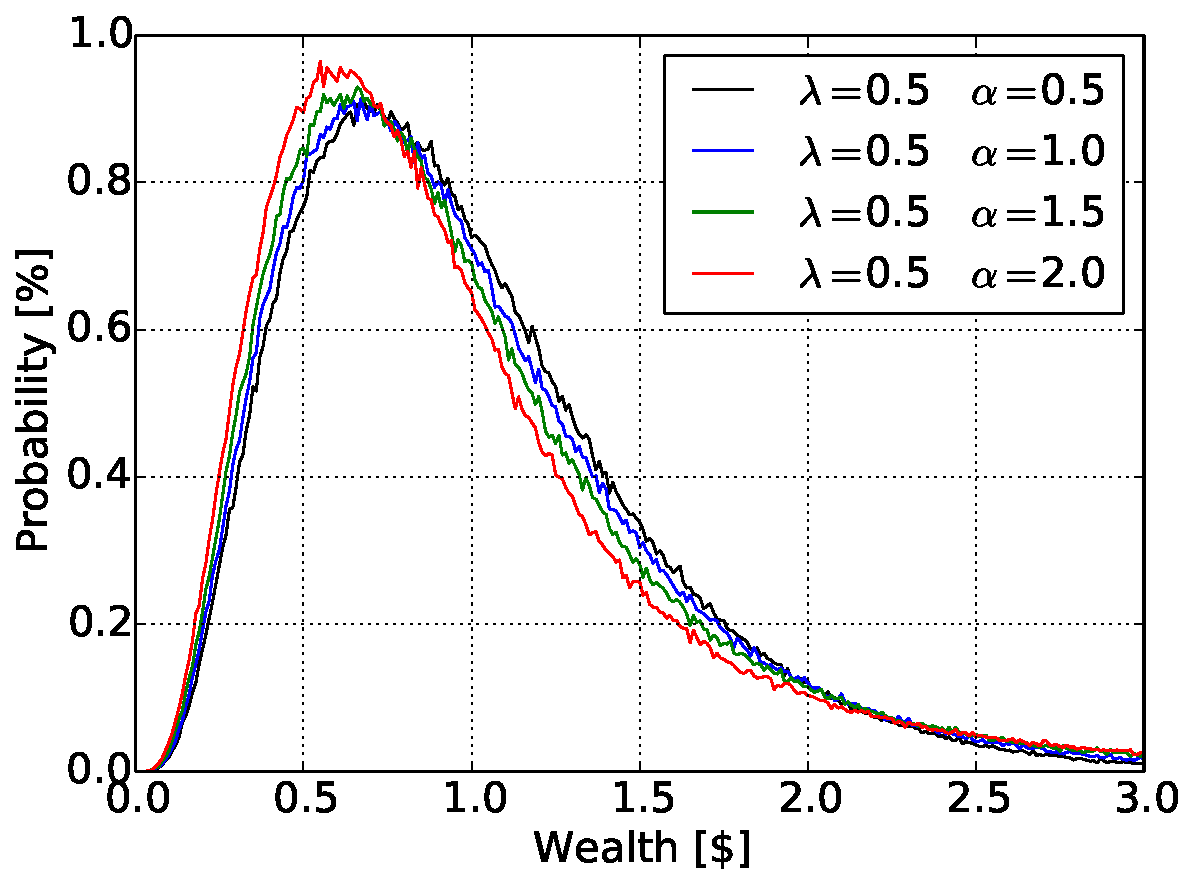
\includegraphics[width=\linewidth]{result/bilder/5d-50}
        \caption{}
    \end{subfigure}%
    ~ 
    \begin{subfigure}{0.5\textwidth}
        \centering
        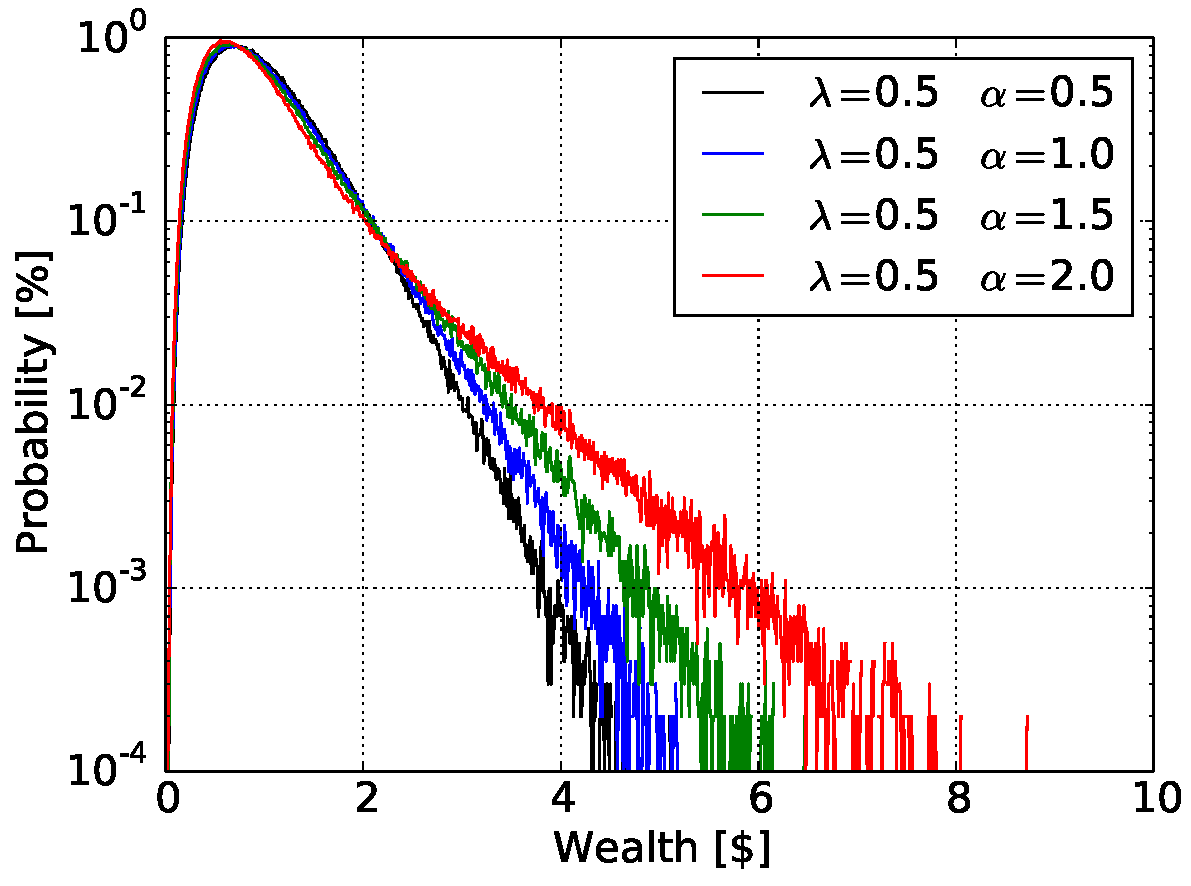
\includegraphics[width=\linewidth]{result/bilder/5d-50-log}
        \caption{}
    \end{subfigure}
    \caption{a) Shows how E behaves around $T_C$ b) Shows how |M| develops near $T_C$.}
    \label{fig:5d-50}
\end{figure}



\begin{figure}[H]
    \centering
    \begin{subfigure}{0.5\textwidth}
        \centering
        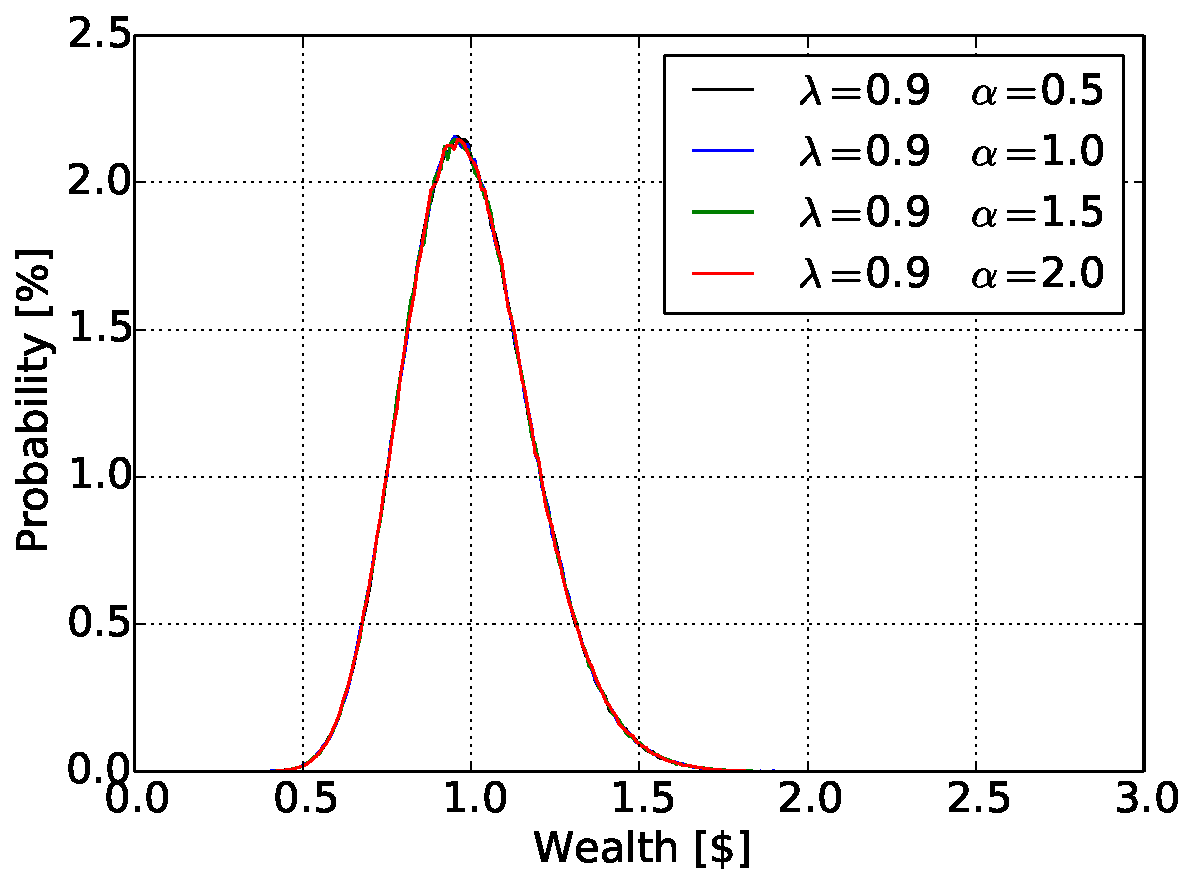
\includegraphics[width=\linewidth]{result/bilder/5d-90}
        \caption{}
    \end{subfigure}%
    ~ 
    \begin{subfigure}{0.5\textwidth}
        \centering
        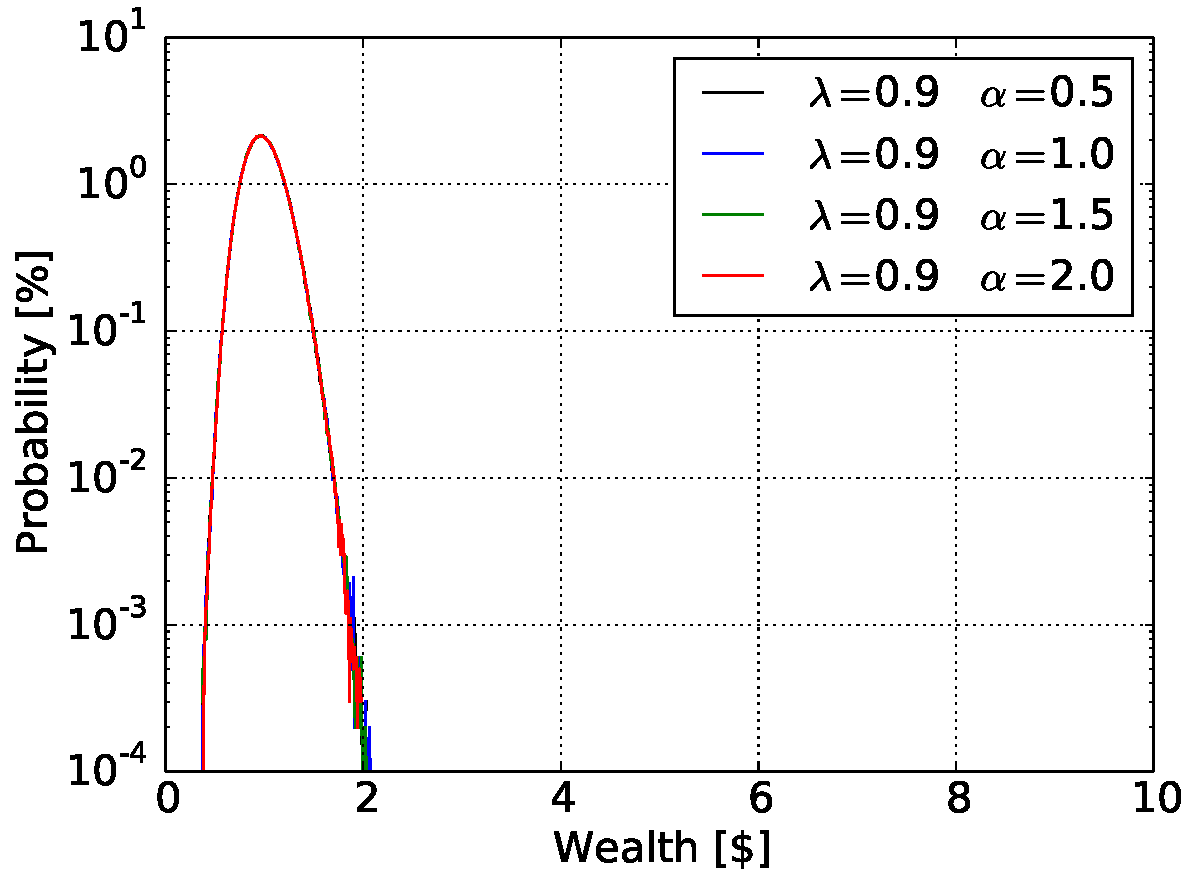
\includegraphics[width=\linewidth]{result/bilder/5d-90-log}
        \caption{}
    \end{subfigure}
    \caption{a) Shows how E behaves around $T_C$ b) Shows how |M| develops near $T_C$.}
    \label{fig:5d-90}
\end{figure}
























\pagebreak
\subsection{5e}
\begin{figure}[H]
    \centering
    \begin{subfigure}{0.5\textwidth}
        \centering
        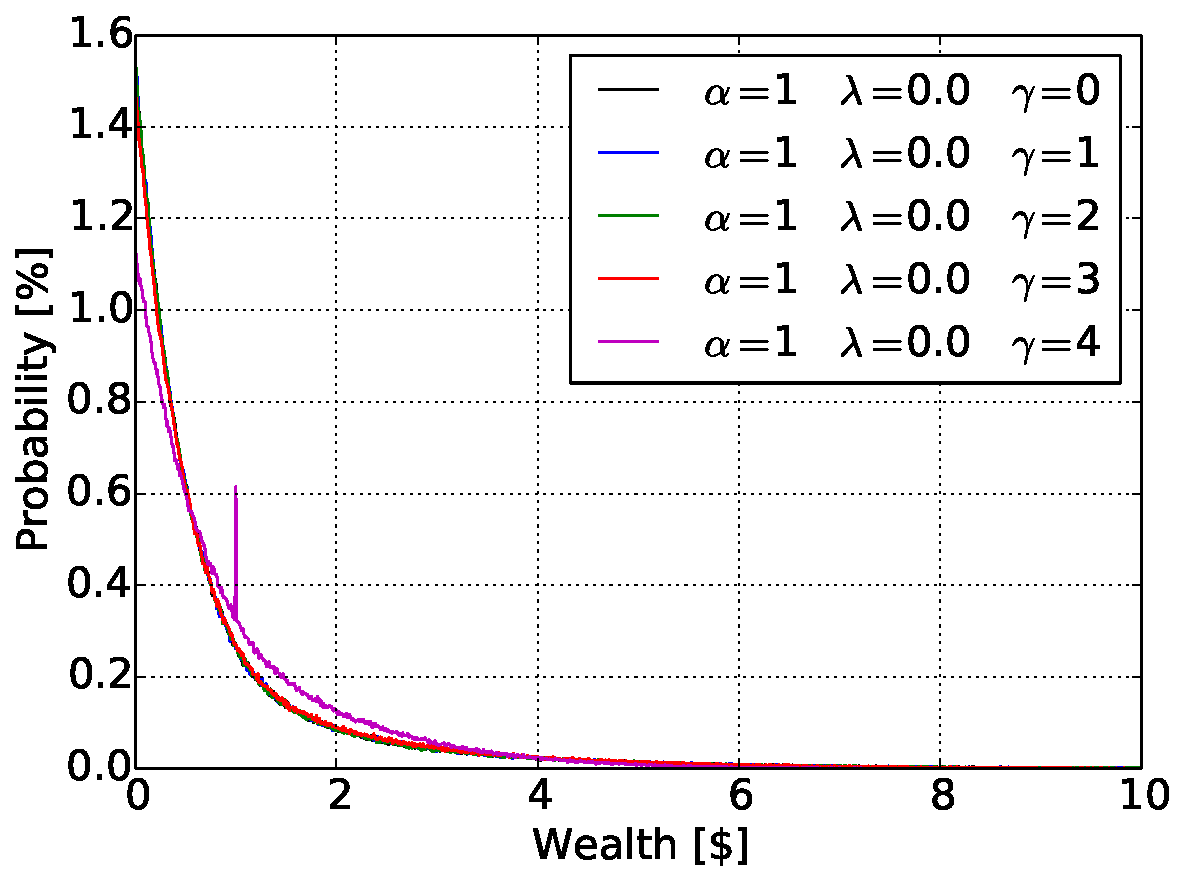
\includegraphics[width=\linewidth]{result/bilder/5e-1-00}
        \caption{}
    \end{subfigure}%
    ~ 
    \begin{subfigure}{0.5\textwidth}
        \centering
        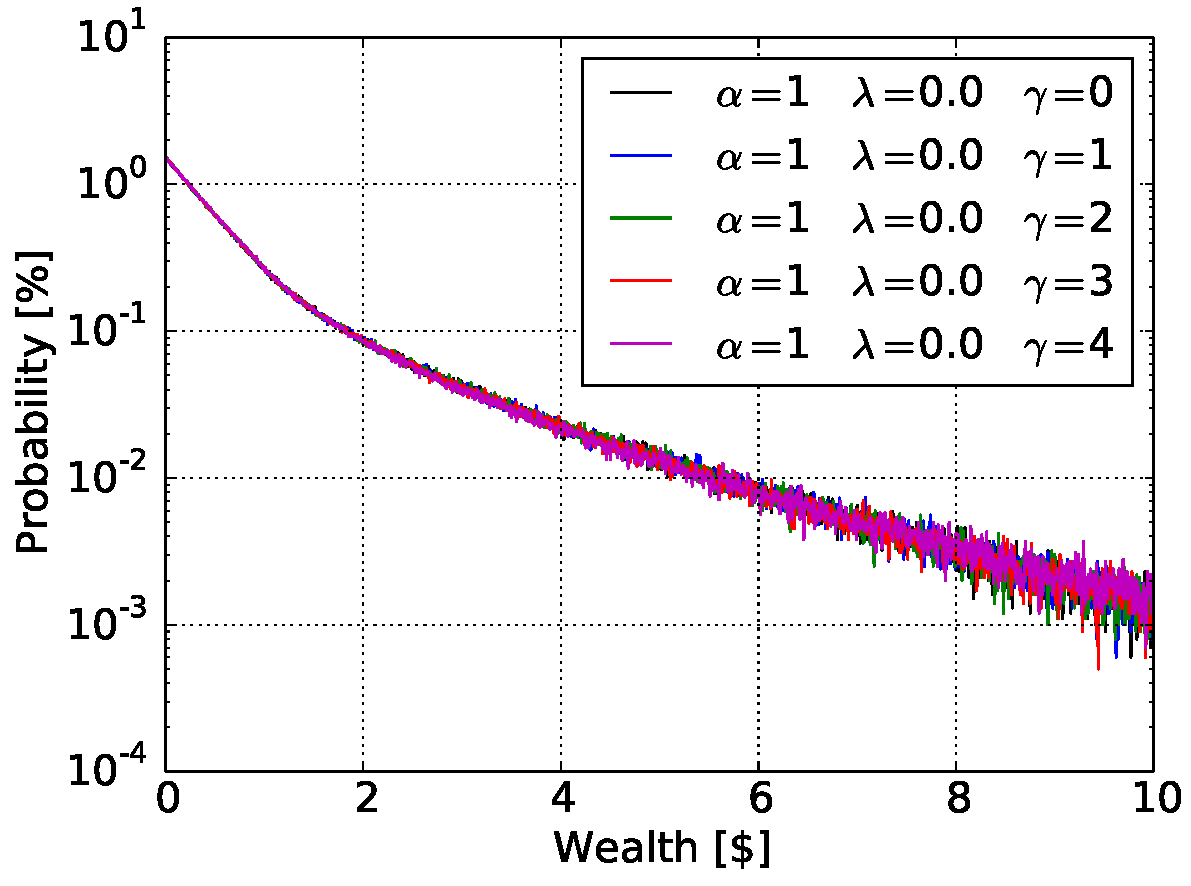
\includegraphics[width=\linewidth]{result/bilder/5e-1-00-log}
        \caption{}
    \end{subfigure}
    \caption{a) Shows how E behaves around $T_C$ b) Shows how |M| develops near $T_C$.}
    \label{fig:5e-1-00}
\end{figure}



\begin{figure}[H]
    \centering
    \begin{subfigure}{0.5\textwidth}
        \centering
        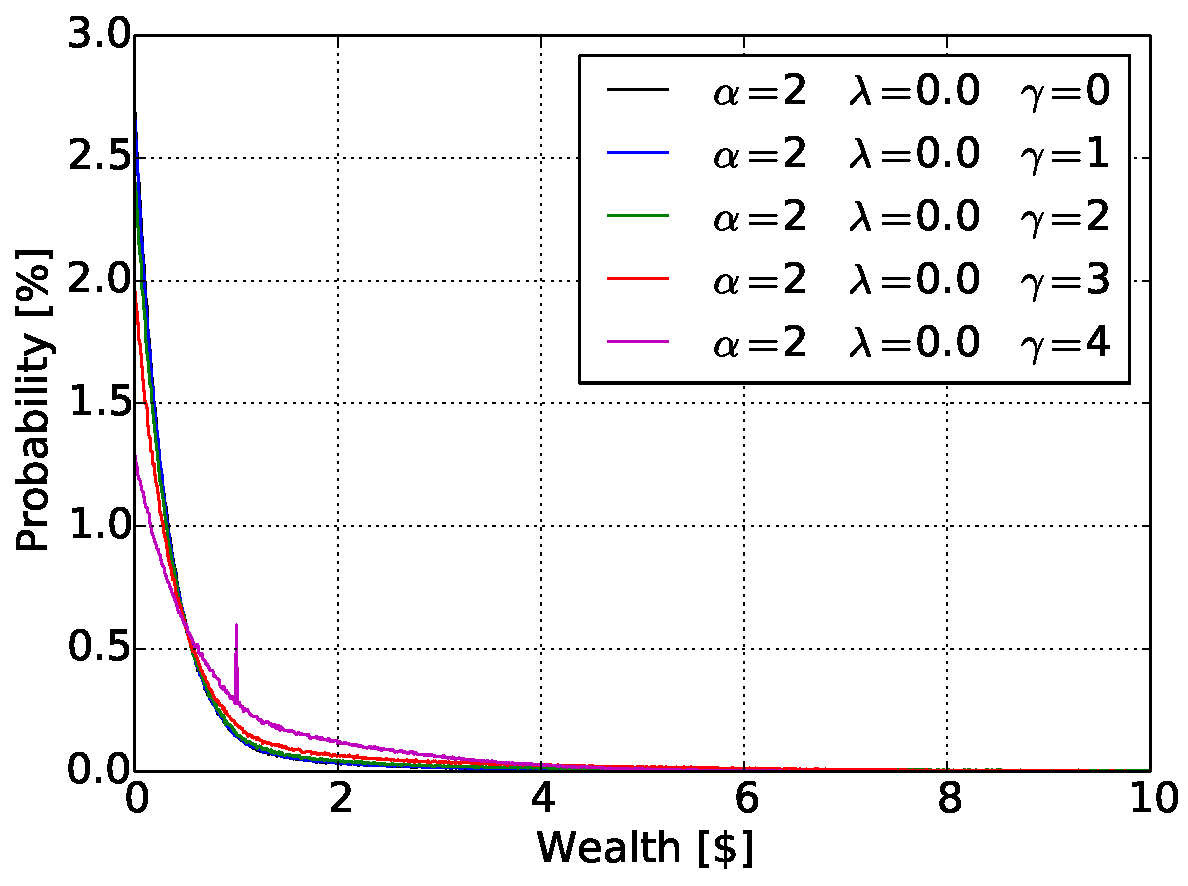
\includegraphics[width=\linewidth]{result/bilder/5e-2-00}
        \caption{}
    \end{subfigure}%
    ~ 
    \begin{subfigure}{0.5\textwidth}
        \centering
        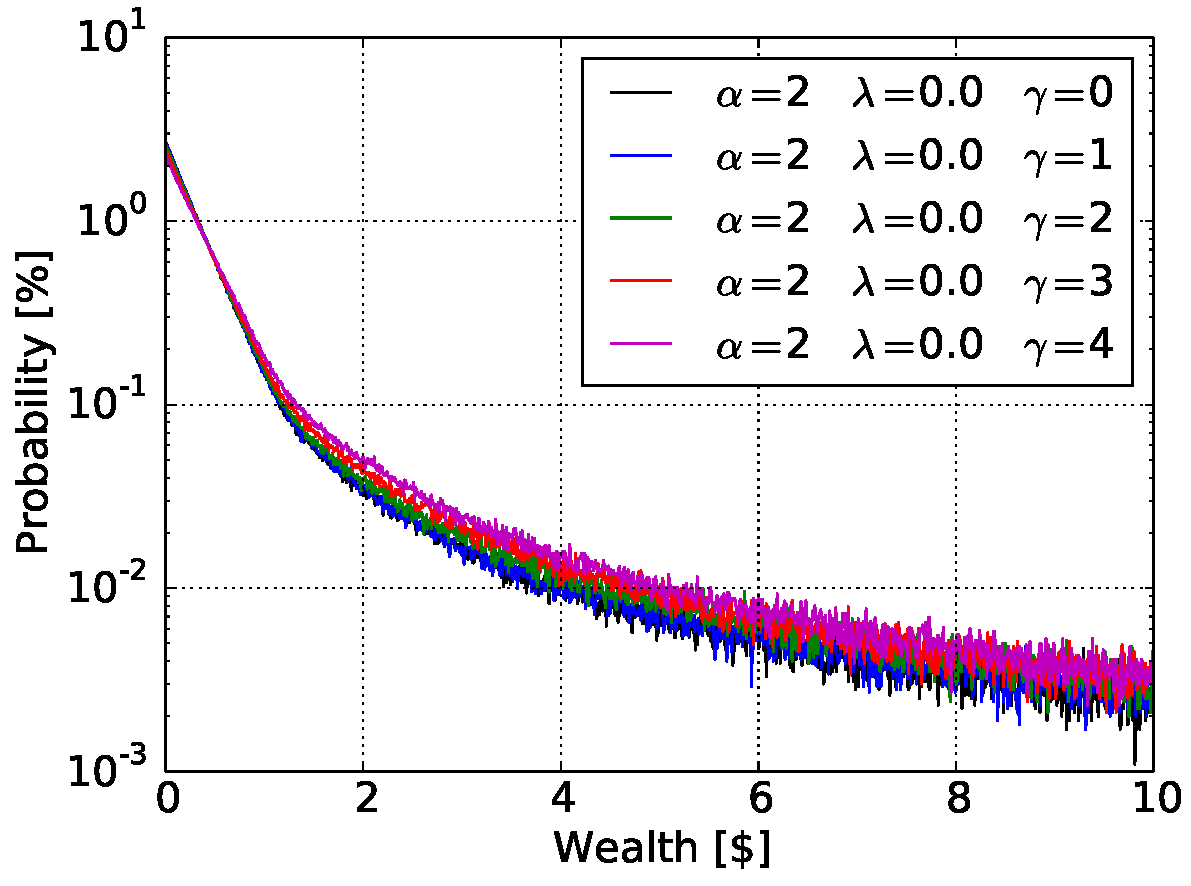
\includegraphics[width=\linewidth]{result/bilder/5e-2-00-log}
        \caption{}
    \end{subfigure}
    \caption{a) Shows how E behaves around $T_C$ b) Shows how |M| develops near $T_C$.}
    \label{fig:5e-2-00}
\end{figure}














\begin{figure}[H]
    \centering
    \begin{subfigure}{0.5\textwidth}
        \centering
        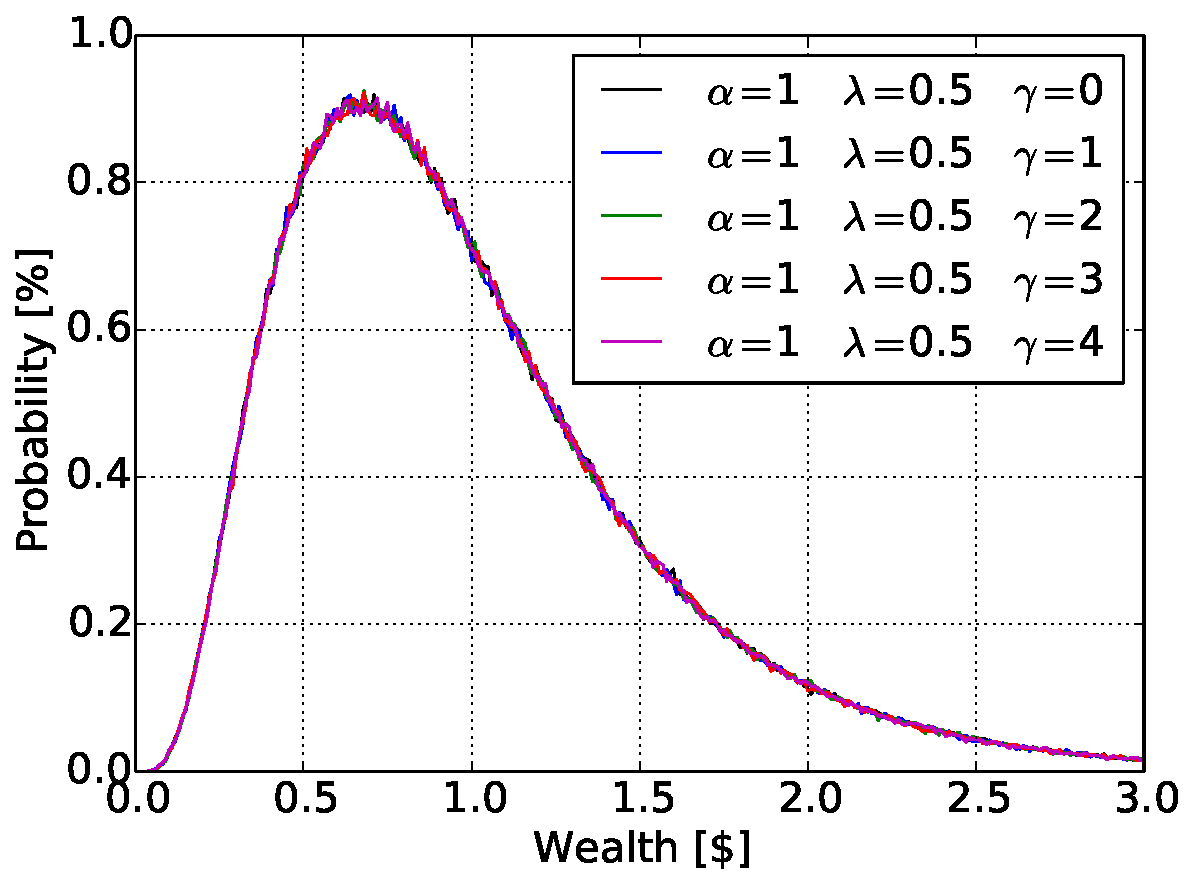
\includegraphics[width=\linewidth]{result/bilder/5e-1-50}
        \caption{}
    \end{subfigure}%
    ~ 
    \begin{subfigure}{0.5\textwidth}
        \centering
        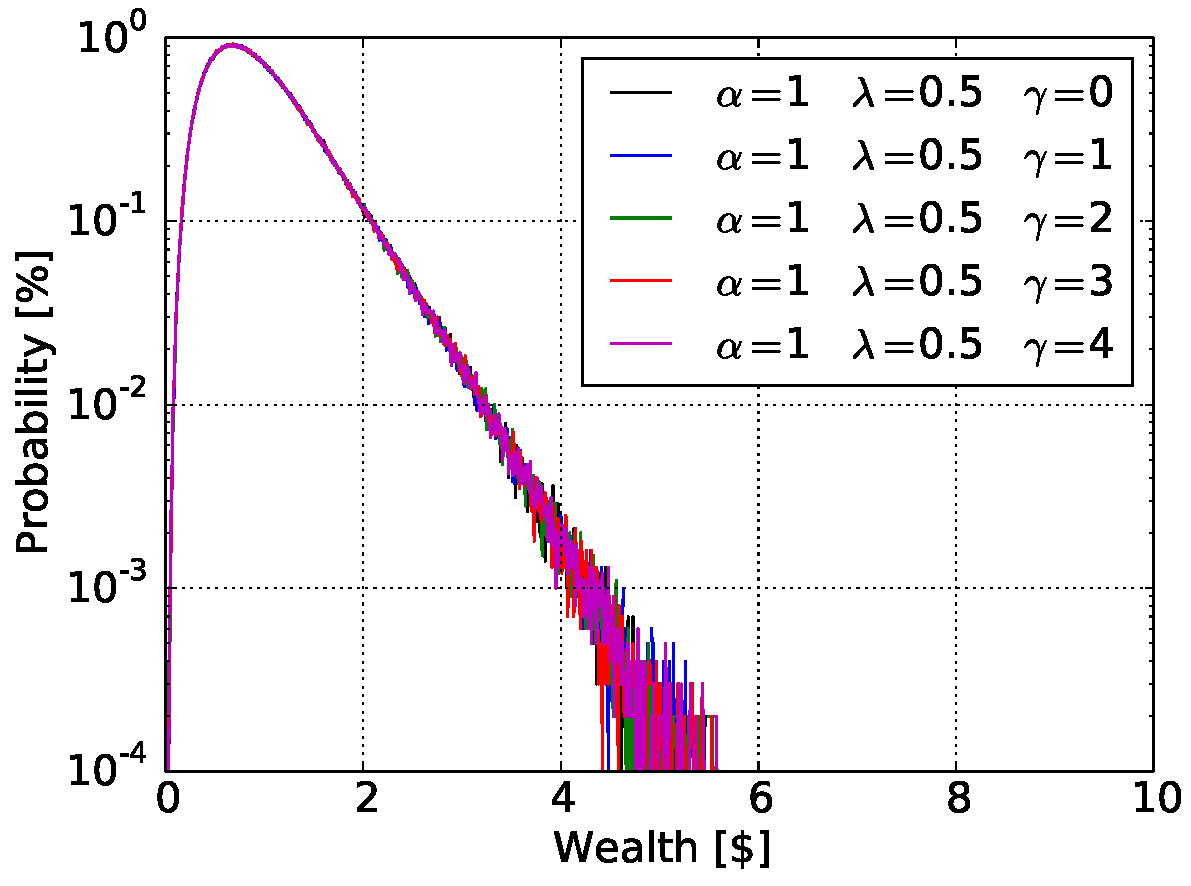
\includegraphics[width=\linewidth]{result/bilder/5e-1-50-log}
        \caption{}
    \end{subfigure}
    \caption{a) Shows how E behaves around $T_C$ b) Shows how |M| develops near $T_C$.}
    \label{fig:5e-1-50}
\end{figure}



\begin{figure}[H]
    \centering
    \begin{subfigure}{0.5\textwidth}
        \centering
        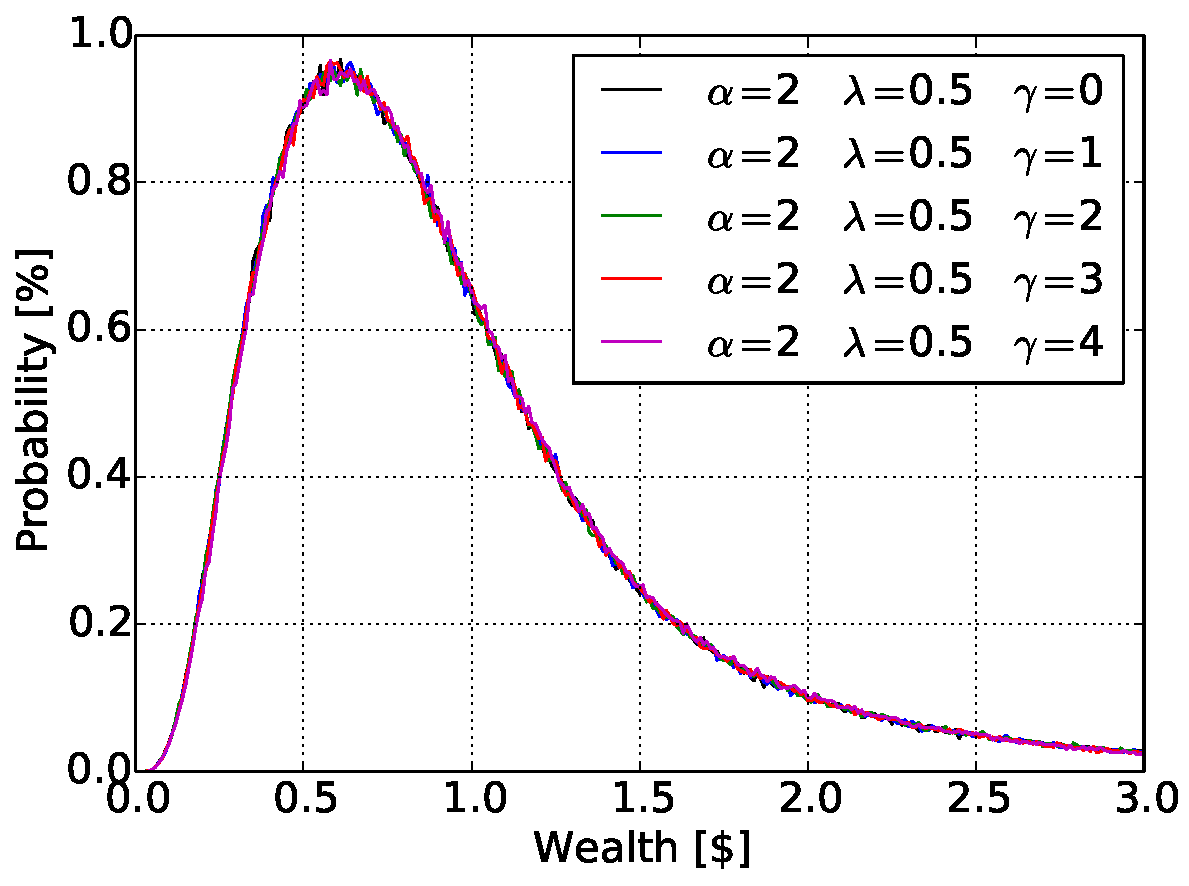
\includegraphics[width=\linewidth]{result/bilder/5e-2-50}
        \caption{}
    \end{subfigure}%
    ~ 
    \begin{subfigure}{0.5\textwidth}
        \centering
        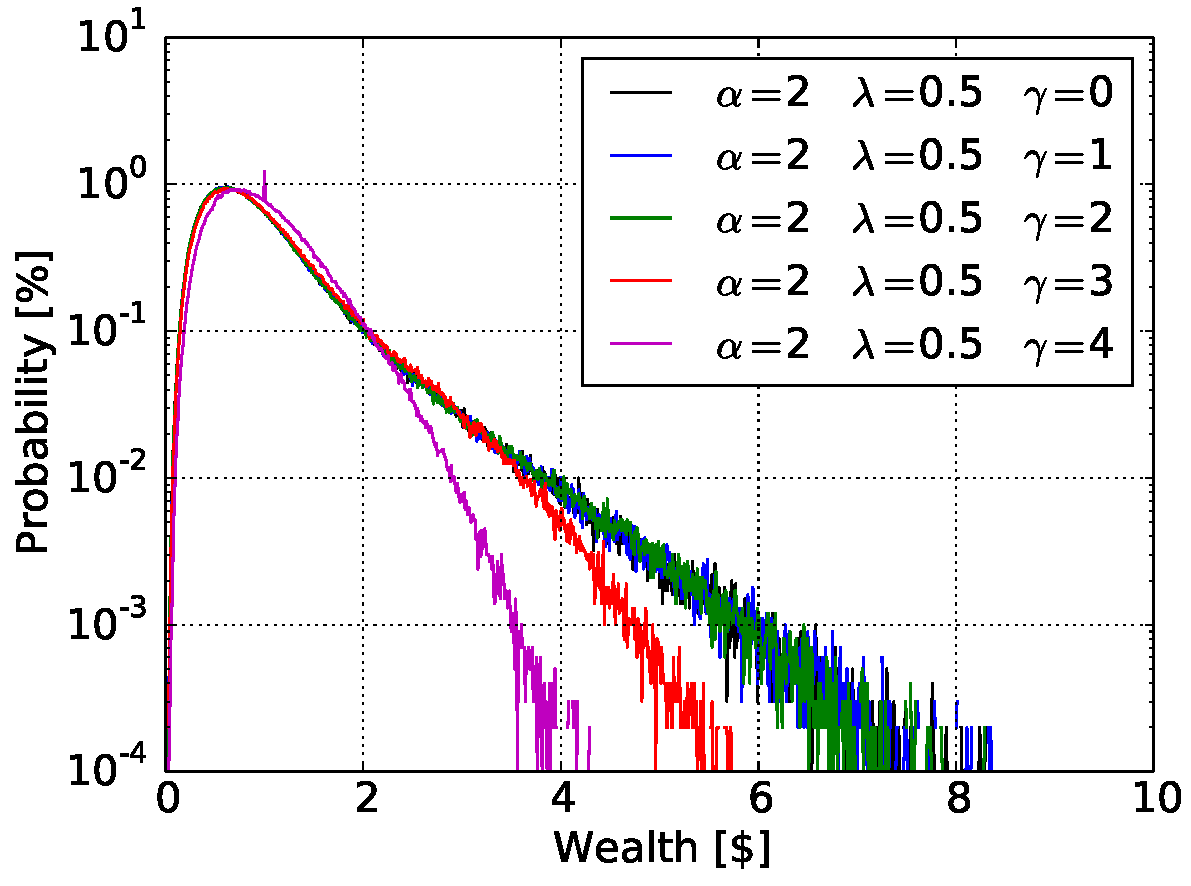
\includegraphics[width=\linewidth]{result/bilder/5e-2-50-log}
        \caption{}
    \end{subfigure}
    \caption{a) Shows how E behaves around $T_C$ b) Shows how |M| develops near $T_C$.}
    \label{fig:5e-2-50}
\end{figure}















\begin{figure}[H]
    \centering
    \begin{subfigure}{0.5\textwidth}
        \centering
        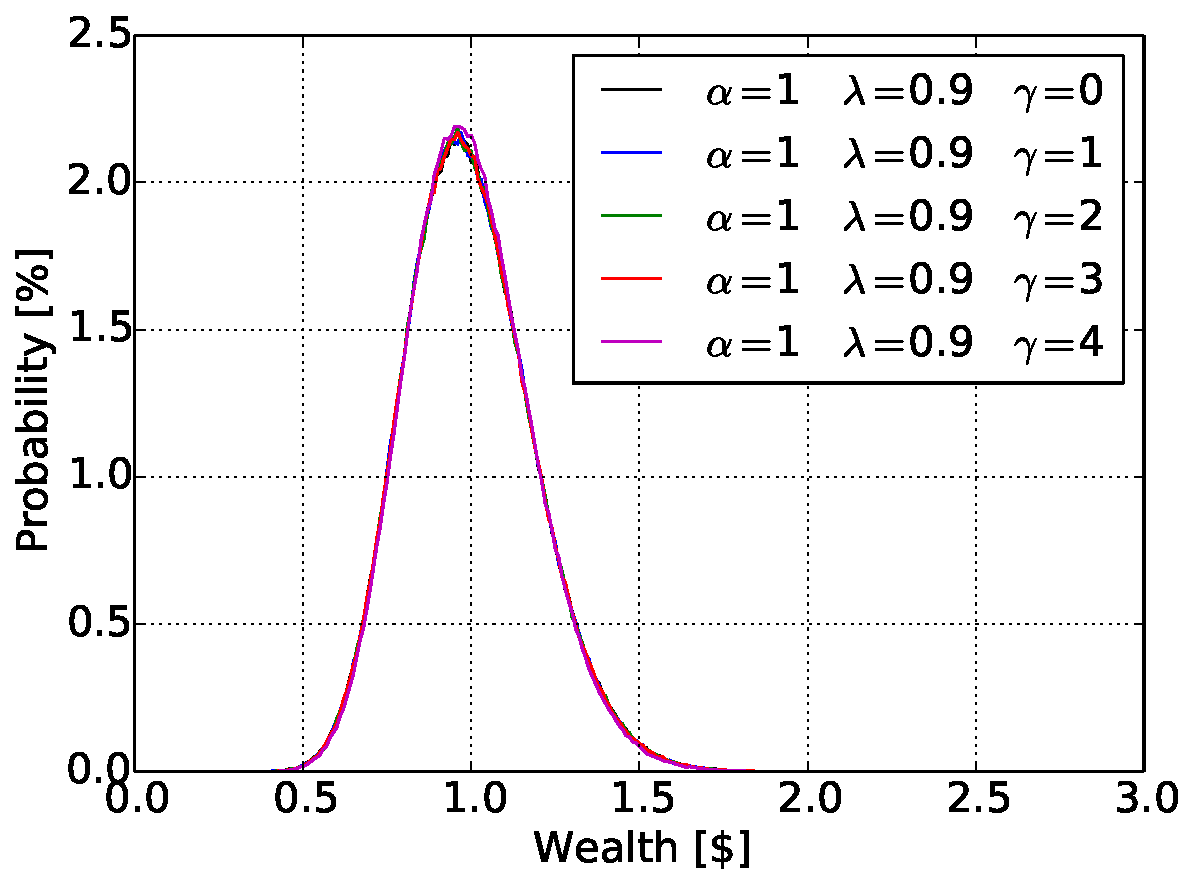
\includegraphics[width=\linewidth]{result/bilder/5e-1-90}
        \caption{}
    \end{subfigure}%
    ~ 
    \begin{subfigure}{0.5\textwidth}
        \centering
        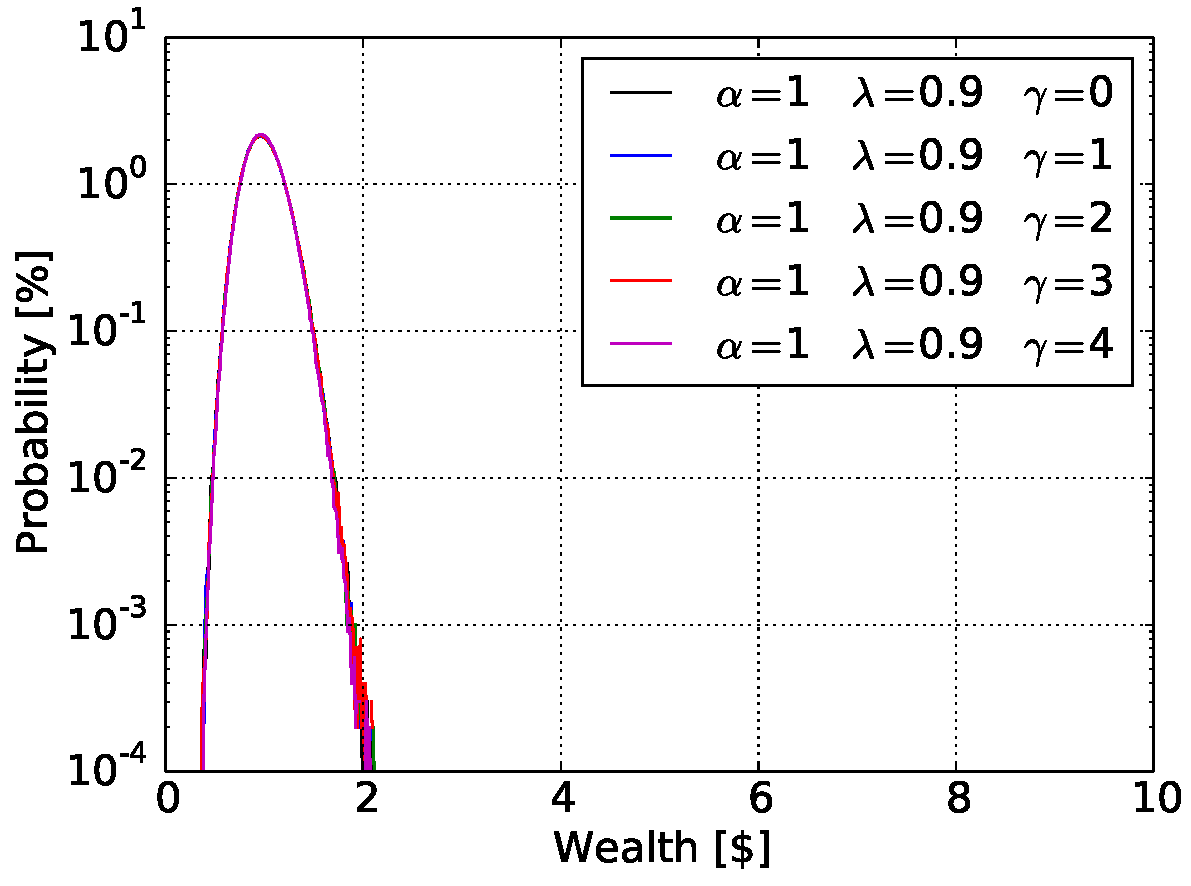
\includegraphics[width=\linewidth]{result/bilder/5e-1-90-log}
        \caption{}
    \end{subfigure}
    \caption{a) Shows how E behaves around $T_C$ b) Shows how |M| develops near $T_C$.}
    \label{fig:5e-1-90}
\end{figure}



\begin{figure}[H]
    \centering
    \begin{subfigure}{0.5\textwidth}
        \centering
        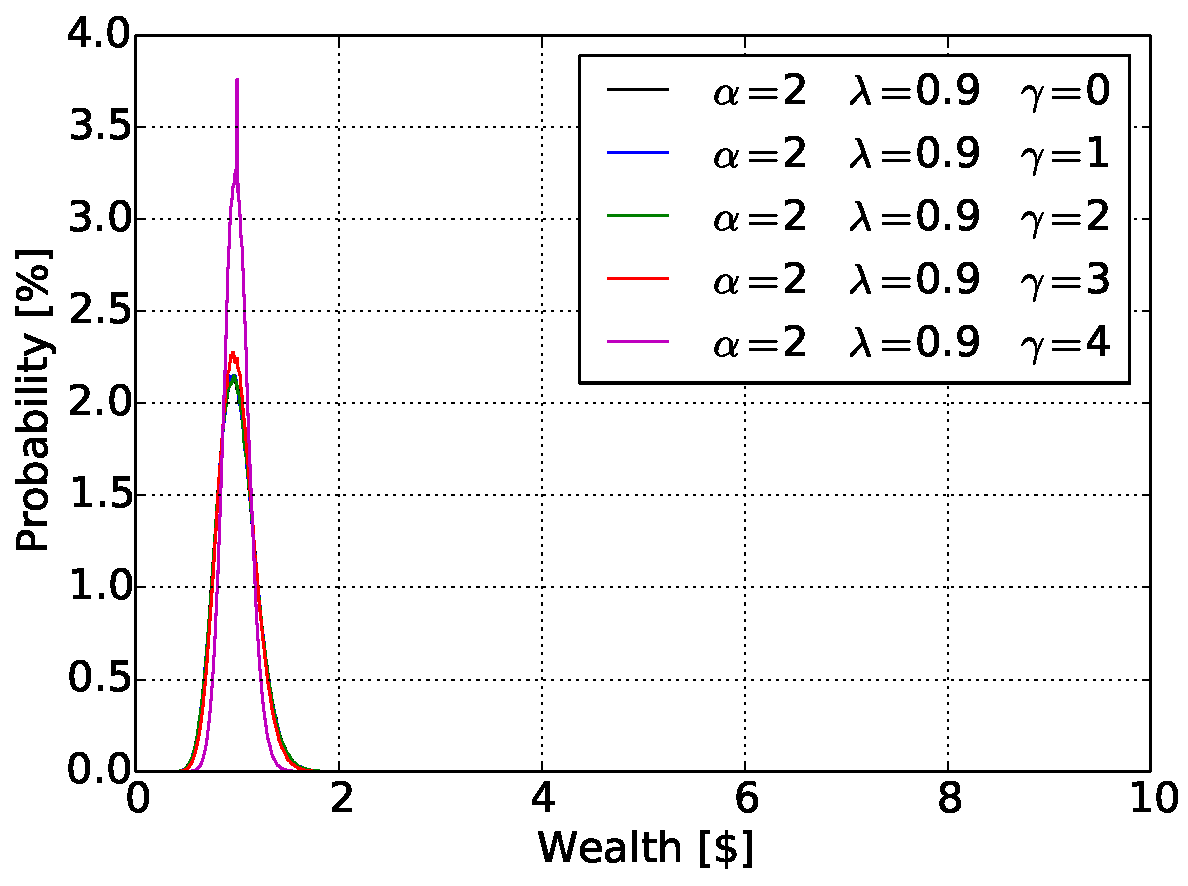
\includegraphics[width=\linewidth]{result/bilder/5e-2-90}
        \caption{}
    \end{subfigure}%
    ~ 
    \begin{subfigure}{0.5\textwidth}
        \centering
        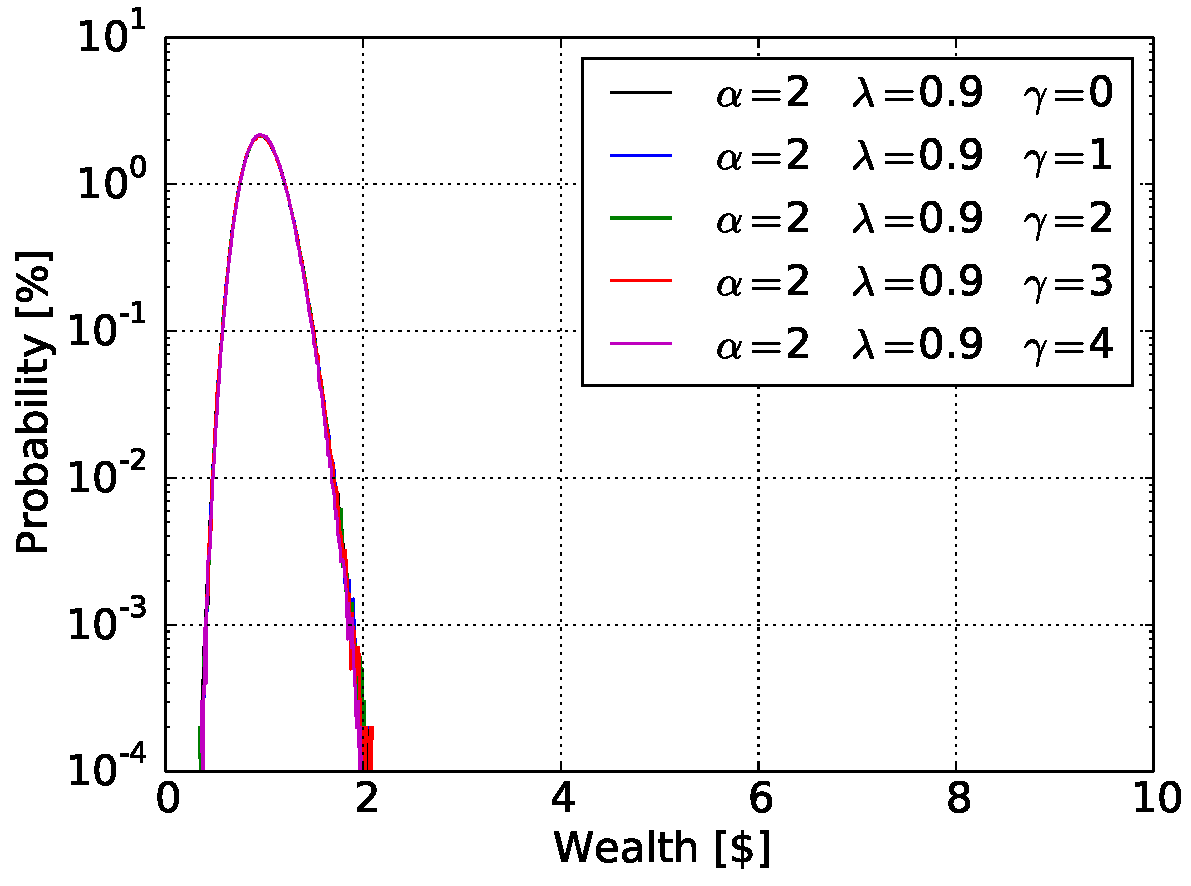
\includegraphics[width=\linewidth]{result/bilder/5e-2-90-log}
        \caption{}
    \end{subfigure}
    \caption{a) Shows how E behaves around $T_C$ b) Shows how |M| develops near $T_C$.}
    \label{fig:5e-2-90}
\end{figure}

















%\pagebreak
%\section{Discussion}
%\input{discussion/discussion}


\section{Conclusion}
In this project a have created a generalized closed transaction model. Agents and the amount of wealth that is traded is randomly selected. A saving term was implemented which turned out to be positive for must agent. Different probability terms were introduced to the model. \todo{MIKAEL, skriv tre setninger om hoved essensen av hva du skrev i resultdelen.}
\\
\\
For future work one should try to make the trade ratio time dependent. The denominator in the trade ratio becomes larger over time, but a more realistic model would make the agents only care about the last part of the transaction they did. The effect of taxing or universal basic income would also be interesting to see, but this was to much work for this project. 

\pagebreak
\section{References}
\printbibliography

\section{Appendix}\label{sec:appendix}
\input{appendix/appendix}



%\begin{align*}
%&n \qquad &2^n - (-1)^n\\
%&n+1 \qquad &2^{n+1} - (-1)^{n+1} \\
%& &= 2(2^{n}) - (-1)^{n+1}\\
%& &= 2(2^{n} + (-1)^n  + (-1)^{n+1}) - (-1)^{n+1}\\
%& &= 2(2^{n} + (-1)^n  - (-1)^{n}) - (-1)^{n+1}\\
%& &= 2(2^{n}- (-1)^{n}) + 2(-1)^n  + (-1)^{n}\\
%& &= 2(2^{n}- (-1)^{n}) + 3(-1)^n \\
%\end{align*}



% \begin{figure}[H]
%     \centering
%     \begin{subfigure}{0.5\textwidth}
%         \centering
%         \includegraphics[width=\linewidth]{result/bilder/Tc/e-Tc}
%         \caption{}
%     \end{subfigure}%
%     ~ 
%     \begin{subfigure}{0.5\textwidth}
%         \centering
%         \includegraphics[width=\linewidth]{result/bilder/Tc/m-Tc}
%         \caption{}
%     \end{subfigure}
%     \caption{a) Shows how E behaves around $T_C$ b) Shows how |M| develops near $T_C$.}
%     \label{fig:tc-E-M}
% \end{figure}






% \begin{center}
% \label{tab:states-2x2-summary}
% \captionof{table}{The table shows a summary from table \ref{tab:states-2x2}. }
% \begin{tabularx}{\textwidth}{c X c X c X c}
%     \hline 
%     \hline 
%         Number of $\color{red}{\uparrow}$ && Multiplicity && Energy && Magnetic moment \\ 
%     \hline
%         4   &&      1      &&      -8J     &&       4       \\  
%         3   &&      4      &&      0J      &&       2       \\
%         2   &&      2      &&      8J      &&       0       \\
%         2   &&      4      &&      0J      &&       0       \\
%         1   &&      4      &&      0J      &&       -2      \\
%         0   &&      1      &&      -8J     &&       -4      \\
%     \hline
% \end{tabularx}
% \end{center}













%\begin{tabular}{|c|c|c|c|c|c|c|}
%	\hline 
%	n & General & Specific & LU & fastest & slowest & $\frac{slowest}{fastest}$\\ 
%	\hline
%	10 & 6.5e-05 & 5e-06 & 4e-05 & Specific & General & 13.0\\ 
%	\hline 
%	100 & 7.5e-05 & 8e-06 & 0.0023 & Specific & LU & 287.5\\ 
%	\hline 
%	1000 & 0.00014 & 4e-05 & 0.26 & Specific & LU & 6500\\ 
%	\hline
%	10000 & 0.0007 & 0.0005 & 142.5 & Specific & LU & 285000 \\ 
%	\hline
%\end{tabular}

%\begin{figure}[H]
%		\centering
%		\includegraphics[width=0.7\linewidth]{ab.png}
%		\caption{Atomene er gule kuler, de elementære vektorene er blå og a vektorene er grønne.}
%		\label{fig:ab}
%\end{figure}



\end{document}
